
Stochastic differential equations are the second core techincal area used in this thesis.
They form the mathematical foundation for dealing processes that evolve randomly through some state space.
The core mathematics of diffusion models are built on top of stochastic differential equations, and so having an understanding of the underlying mathematical tools is helpful for making advances.

In this chapter I aim to give a gentle introduction to the formalisation of stochastic differential equations.
To do so, I first intrduce the measure theory formalisation of probability theory, nessicary for dealing with probabilites on infinite-dimension spaces.
Next, I provide an introduction to the formalisation of stochastic differential equations, including various definitions of stochasitc integrals and methods for working with them.
Finally I highlight a number of results with simple proofs that are very useful in formalsing diffusion models.

\section{A review of measure theory based probability}
It is neccisary when talking about stochastic processes to work with probability under the \emphmarginnote{measure theory} approach.
Without this, there is no clear way to discuss probability on infinite dimension spaces, such as the space of continuos functions on interval \(\sbr{0,1}\). 
There are a number of other otivations for studying measure thoery, particualrly concerning techicaly difficulties that arise with the usual definitions of probability that one encounters.
Examples of such motivations can be found in ....

The presentation is based on \textcite{kallenberg1997foundations}, and takes inspiration from \textcite{terenin22}.

A \emph{\(\sigma\)-algebra}, much like a topology, is a collection of sets obeying a set of rules.
The definition even looks very similar.
But this is where the similarity ends.
\begin{definition}[Measurable space]
	A measurable space (\(X, \sigalg{X}\)) is a set \(X\) along with a collection of subsets \(\sigalg{X}\) of \(X\), called a \emphmarginnote{sigma/\(\sigma\)-algebra}, that satisfy the following:
	\begin{itemize}
		\item \(X \in \sigalg{X}\), and is called the \emph{universal set}.
		\item \(\sigalg{X}\) is closed under \emph{compliments}.
		\item \(\sigalg{X}\) is closed under \emph{countable} unions.
	\end{itemize}
\end{definition}
From this it also follows that a \(\sigma\)-algebra is closed under countable intersections, and that \(\emptyset \in \sigalg{X}\).

The definition of a \(\sigma\)-algebra means that it contains within itself the limits of any sequence of sets contained in it, which allows us to define some sensible concepts of convergence of random variables, to be discussed later.

Of particular relevance are \emphmarginnote{Borel \(\sigma\)-algebras\label{def:borel_sigma_algebra}}.
For a topological space \((X, \topo{X})\), the Borel \(\sigma\)-algebra, \(\c{B}\del{(X, \topo{X})}\) is the smallest sigma algebra containing the topolog \(\topo{X}\). \todo{manifold boreal are the volume form ones go look at forre}

A \emphmarginnote{measure\label{def:measure}} on a measureable space is a function \(\mu: \sigalg{X} \to \R\) that is also non-negative, is zero on the empty set, and is countably additive.
This is that for disjonit sets \(\E_1,...  \in \sigalg{X}\), \(\mu\del{\U_i E_i} = \sum_i  \mu(E_i)\).
With this in mind we can intepret the \(\sigma\)-algebra as the set of sets we can measure.
The restriction we place on this set of measurable sets is exactly designed to avoid techincal issues that can appear.
For example, on the real numbers \(\R\) for a particular subset \(\sbr{a,b}\) we would make this simply \(|b-a|\).
In this way, we are leasuring the length of this set.
A \emphmarginnote{measure space} is a measurable space along with a metric, \((X, \sigalg{X}, \mu)\).

We can take \emphmarginnote{products of measureable spaces}.
For a countable sequance of spaces \((X_i, \sigalg{X_i})_{i=1}^\infty\) the \emphmarginnote{product \(\sigma\)-algerba} \(\bigotimes_i \sigalg{X_i}\) is given by the smallest \(\sigma\)-algebra containing the \emph{cylendar sets} (\cref{eq:cylendar_sets}) of the \(\sigalg{X_i}\).
Note the similarity to the definition of the product topology.
Indeed for \emph{Hausdorff} (\cref{def:hausdorff}) (and other types of seperablity) the product \(\sigma\)-algebra and the product topology interact nicely.
\[
	\c{B}\del{\prod_i (X_i, \topo{X_i})} = \bigotimes_i \c{B}\del{(X, \topo{X})}
\]

A function \(f: X\to Y\) between two measureable spaces, \((X, \sigalg{X})\), \((Y, \sigalg{Y})\), \(f:X \to Y\) is said to be a \emphmarginnote{measurable function}, denoted \(\sigalg{X}/\sigalg{Y}\)-measurable, if for any \(U \in \sigalg{{Y}}\), \(f^{-1}(U)\in \sigalg{X}\).
This says if I can measure a set in \(Y\), then I can measure its preimage in \(X\). Notice again the similiarity to this definition to the definition of continuity. Indeed for any pair of topological spaces with the Borel \(\sigma\)-algebra, \((X, \topo{X}, \c{B}(\topo{X}))\), \((Y, \topo{Y}, \c{B}(\topo{Y}))\), any continuout function \(f:X\to Y\) is \(\c{B}(\topo{X})/\c{B}(\topo{Y})\)-measureable. Like continuous functions, the \emphmarginnote{composition} of measureable functions is again measurable.

For \emphmarginnote{measureable functions on product spaces} the function \(f: X\to Y\times Y'\) is \(\sigalg{X}/\sigalg{Y}\otimes\sigalg{Y'}\)-measureable if each component function is measureable. The conversere is \emph{not} true.  \(f: X\times X'\to Y\) is not nessicarily measureable if \(f(\cdot, x'): X\to Y\) and \(f(x, \cdot): X'\to Y\) are measurable.

A \emphmarginnote{probability measure} is a measure \(\mu: X\to \R\) on a measureable space \((X, \sigalg{X})\) such that \(\pi_X(X) = 1\).
A \emphmarginnote{probabilty space}, \((\Omega, \c{F}, \P)\) in standard notation, is a measurable space along with a probability measure.
In this way, we can think about \(\c{F}\) as the set of sets of events \(A_\omega \subset \Omega\) that we can ask questions about probability about.
We are preculded from asking questions about sets that are not in \(\c{F}\) as it creates techincal issues.
In this sense a probability measure describes the uncertainty we have about the events \(\omega \in \Omega\).
Typically when dealing with probabiities, the space \(\Omega\) is very abstract, and we simply choose one with "enough elements" and a \(\sigma\)-algebra with enough sets in be able to achive what we want to. 
We can see \(\Omega\) as a bag of random numbers and \(\P\) as a random generator function from this bag, not dissimliar to a random number generator influencing events in a computer simulation.

We define a \emphmarginnote{random variable} as a measurable function \(x: \Omega \to X\) from a probability space into a measurable space. 
A random variable can then be thought as mapping abstract randomly generated events \(\omega \in \Omega\) into real observations in \(X\).
The \emphmarginnote{distribution of a random variable} is given by \(\pi_x = x^*\P\), where this denotes the \emph{pushforward} of \(\P\) through \(x\), defined by \((x^*\P)(A_x) = \P(x^{-1}(A_x))\) for \(A_x\in \sigalg{X}\).
The probabilty of a collection of events \(A_x\) happening in \(X\) is then the probabiity of their preimage happening in \(\Omega\).
The fact that \(x\) is measurable guarentees this is well defined.

\marginnote{The existence of random variables}To expand on the point of being able to choose \(\Omega\) to include enough events to be interesting, it is not guarenteed that for a given proabilty space \((\Omega, \c{F}, \P)\) and distribution \(\pi_x\) that there exists a random variable \(x: \Omega \to X\) such that \(\pi_x = x^*\P\). 
However, given a \(\pi_x\) and a proabilty space \((\Omega, \c{F}, \P)\) it is possible to find a \emph{bigger} probability space \((\Omega', \c{F}', \P')\) along with a measureable surjection \(i: \Omega' \to \Omega\) such that \(i_* \P' = \P\) and a random variable \(x: '\Omega \to X\) exists with distribution \(\pi_x\).

The \emphmarginnote{expectation} of a random variable is only defined is the space of the random variable has enough structutre\todo{what structure?}. For real valued random variables, \(x:\Omega\to \R\), we can equip \(\R\) with ... and so the expectation \(\E\sbr{x}\) can be thought of as the weighted average value of \(x\) under the values of \(x\) generated by \(\P\). For a suitable notion of integration, namely Lebesgue integration, this is
\[\E\sbr{\mathsf{X}} = \int_X x \d \pi_{\up{X}}(x) = \int_\Omega \mathsf{X}(\omega) \d\P (\omega)\]
where this integration happens against the measure \(\pi_x\).

For \emphmarginnote{manifold-valued random variables}, \(x:\Omega\to M\), however this structure is rarely presents, and so the expectation is undefined.
In order to study such random variables we often look at their behaviour under composition with measurable test functions \(f: M \to \R\) as we can then take the expectation of the random variable \(f\circ x : \Omega\to \R\).
This definition of expection applies clearly to real vector-valued random variables as well.

The \emphmarginnote{covariance} of a pair of random variables, if it exisits, is then given by \(\Cov\del{x, x'} = \E\sbr{xx'} - \E\sbr{x}E\sbr{x'}\).
This definition also extends to real vector-valued random variables as well by applying it component-wise.

For a pair of random variables, \(\up{X}\), \(\up{X}'\) on a measurable space \((X, \sigalg{X})\) relative to a probability space \((\Omega, \c{F}, \P)\), we can define equality in a number of ways.
We say that they are \emphmarginnote{equal surely}, denoted \(\up{X} = \up{X}'\), if \(\up{X}(\omega) = \up{X}'(\omega)\) for all \(\omega \in \Omega\), i.e. they are equal as functions.
As it turns out this definition is generally too strict.

We say that they are \emphmarginnote{equal almost-surely}, denoted \(\up{X} = \up{X}' \as \), if \(\P(\up{X} = \up{X}') = 1\).
This means that they agree as functions \emph{except} on sets of probability zero.
Almost-sure equality is implied by sure equality.

Weaker than this, but still maintaining the , we say that two random variables are \emphmarginnote{equal in distribution}, denoted \(\up{X} \overset{d}{=} \up{X}'\), if the measures \(\pi_{\up{X}} = \up{X}_*\P\) and  \(\pi_{\up{X}'} = \up{X}_*'\P\) are equal.
In other words this implies that \(\up{X}(A) = \up{X}'(A) \; \forall A\in \sigalg{X}\).
This means that they assign the same probabilities to events in \(X\), but these events may \emph{not} have been generated by the same random events in \(\Omega\).
Equality in distribtion is implied by almost-sure equality.

\begin{figure}
	\centering
	\hspace{0.5in}\documentclass[tikz,10pt]{standalone}
\usepackage[standalone,commands]{../../MJH}

\graphicspath{/Users/mhutchin/Documents/thesis/figures/diagrams/}

% \usepackage{tikz}
% \usetikzlibrary{positioning}

\usepackage{pgfplots}
\pgfplotsset{compat=1.17}
% \usepgfplotslibrary{external}
% \usepgfplotslibrary{groupplots}
% \usepgfplotslibrary{fillbetween}
% \usetikzlibrary{fadings}
\usetikzlibrary{fit,calc,trees,positioning,arrows,shapes,calc}

\begin{document}
    % \tikzsetnextfilename{generative_model}
    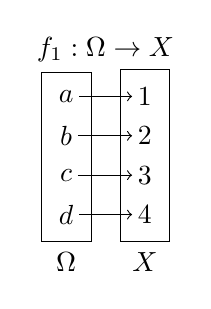
\begin{tikzpicture}[every fit/.style={rectangle,draw,inner sep=1mm,}]
        \node[] (a) at (0,1.5) {$a$};
        \node[] (b) at (0,1.0) {$b$};
        \node[] (c) at (0,0.5) {$c$};
        \node[] (d) at (0,0.0) {$d$};
        \node[] (omega) at (0,-0.6) {$\Omega$};

        \node[] (1) at (1,1.5) {$1$};
        \node[] (2) at (1,1.0) {$2$};
        \node[] (3) at (1,0.5) {$3$};
        \node[] (4) at (1,0.0) {$4$};
        \node[] (x) at (1,-0.6) {$X$};

        \node [] (f) at (0.5,2.1) {$f_1:\Omega \to X$};
        

        \node[draw,fit= (a) (d)] {};
        \node[draw,fit= (1) (4)] {};

        \draw[->,shorten <=-0.5mm,,shorten >=-0.5mm] (a) -- (1) {};
        \draw[->,shorten <=-0.5mm,,shorten >=-0.5mm] (b) -- (2) {};
        \draw[->,shorten <=-0.5mm,,shorten >=-0.5mm] (c) -- (3) {};
        \draw[->,shorten <=-0.5mm,,shorten >=-0.5mm] (d) -- (4) {};

    \end{tikzpicture}
\end{document}\hfill\input{figures/tex/random_variable_equality_y.tex}\hfill \input{figures/tex/random_variable_equality_z.tex}\hspace{0.5in}
	\caption{Consider random variables \(f_1,f_2,f_3\), with \(\Omega=\cbr{a,b,c,d}\) and \(X=\cbr{1,2,3,4}\). Since this is a finite set, we can make the \(\sigma\)-algebra \(\c{F}\) the power set (the set of all subsets) of \(\Omega\) (this does not work on uncountable spaces like \(\R\)
	), and the same for \(\sigalg{X}\). Let \(\P(\cbr{a}) = \P(\cbr{b}) = 0.5\) and \(\P(\cbr{c}) = \P(\cbr{d}) = 0\). Clearly then \(f_1,f_2, f_3\) are equal to themselves surely. \(f_1\) and \(f_2\) are equal almost surely as the only sets they don't agree on are \(\cbr{c}, \cbr{d}\), and these are measure 0 under \(\P\). \(f_1,f_2\) are equal to \(f_3\) in distribution only. The measures \(\pi_{f_1}, \pi_{f_2}, \pi_{f_3}\) all assign the same probabilites to sets of \(X\) (\(\pi_f(\cbr{1}) = \pi_f(\cbr{2}) = 0.5\), \(\pi_f(\cbr{1,2}) = 1\),  \(\pi_f(\cbr{3}) = \pi_f(\cbr{4}) = 0.0\), etc ), but the are not the same as functions on sets of non-zero measure, (\(f{1,2}(\cbr{a}) \neq f_3(\cbr{a})\), \(f_{1,2}(\cbr{2})\neq f_3(\cbr{2})\))}
\end{figure}

These notions of equality also lead to definitions of limits of sequences of random variables.
Let us consider a random variable \(X\) and a sequence of random variables \(\del{X_n}_{n=1}^\infty\) on a proabilty space \((\Omega, \c{F}, \P)\).

\emphmarginnote{Sure convergence} or \emphmarginnote{pointwise convergence} implies that \(X_n\) converges as a function to \(X\), that is
\[
	\lim_{n\to\infty} X_n(\omega) = X(\omega)\;\forall\;\omega\in\Omega, \quad \text{and is denoted by} \quad X_n \to X
\].
As before, this notion is often too strong, and so we define \emphmarginnote{almost sure convergence} as
\[
	\P\del{\lim_{n\to\infty} X_n = X} = 1, \quad \text{and is denoted by} \quad X_n \overset{\as}{\to} X
\]
which means that \(X_n\) need not converge to \(X\) on sets of measure zero.
Almost-sure convergence is implied by sure converge

If \(X\) has metric space structure we can define \emphmarginnote{convergence in proabilty\label{def:probability-converge-rv}} as, for all \(\epsilon\)
\[
	\lim_{n\to\infty}{\P\del{d\del{X, X_n} \geq \epsilon}} = 0, \quad \text{and is denoted by} \quad X_n \overset{p}{\to} X
\].
convergence in proabilty is implied by almost-sure convergence.

We define \emphmarginnote{convergence in distribution\label{def:distribution-converge-rv}} as
\[
	\lim_{n\to \infty} \P\del{X_n\in A} = \P\del{X\in A}, \quad \text{and is denoted by} \quad X_n \overset{L^p}{\to} X
\].
Convergence in distribtion is implied by convergence in proabilty.

Finally, if we have stucture that allows for expectations we can define \emphmarginnote{convergence in \(L^p\)-norm\label{def:l2-converge-rv}}, if \(\E\sbr{\norm{X_n}_p^p}\) and \(\E\sbr{\norm{X}_p^p}\) exist, as
\[
	\lim_{n\to\infty} \E\sbr{\norm{X_n - X}_p^p} = 0, \quad \text{and is denoted by} \quad X_n \overset{\as}{\to} X
\].
Convergence in \(L^p\) for \(p\geq1\) implies convergence in probability, and is usually easier to work with directly.

\subsubsection{Interactions between random variables}
We will need often to work with the interaction between one or more random variables.

Consider a joint random variable \(\mathsf{Z}: \Omega \to X \times Y\), a \(\c{F}/\sigalg{X}\otimes \sigalg{Y}\) measurable function, with distribution \(\pi_{\mathsf{Z}}:X \x Y \to \R\).

The \emphmarginnote{marginal random variable} \(\mathsf{X}: \Omega \to X\) is given by \[\proj_X\circ \mathsf{Z}: \Omega \to X, \quad \text{ where } \proj_X: X\times Y \to X, \; (x, y) \mapsto x\], where the \(\proj_X\) function projects onto the \(X\) coordinate. 
We can create from the \emphmarginnote{marginal distribution} \(\pi_{\mathsf{X}}:X\to\R\), given by \[\pi_{\mathsf{X}}(A_X) = \pi_{\mathsf{Z}}(A_X\x Y), \; A_X\in\sigalg{X}\].

A \emphmarginnote{probability kernel} is a function \(\pi_{\mathsf{X} | \mathsf{Y}}: \sigalg{X}\times Y \to \R\) is a function that 1) \(\pi_{x|y}(\cdot \given y): X\to \R\) is a probability measure and 2) \(\pi_{x|y} (A_x \given \cdot):Y\to\R\) is \(\sigalg{Y}/\c{B}(\R)\)-measureable. These are useful for a few reasons, defining stochastic processes, but also conditional distributions. 

We define the \emphmarginnote{conditional distribution}, \(\pi_{x|y}:X\times Y\to \R\), where it exists, as the unique probability kernel satisfying
\[\pi_{x, y}(A_x \times A_y) = \int_{A_y} \pi_{x|y}(A_x | y) \d\pi_y(y)\]
where \(\pi_{x,y}\) is a joint distribution and \(\pi_y\) is the marginal distribution of \(y\).

This can also be viewed from the perspective of \emphmarginnote{disintegration of a measure}.
\cite{chang1997conditioning}\todo{I quite liked this as a perspective on conditional probability}

\subsubsection{Densities}
When we have two measures on the same measurable space \((X, \sigalg{X})\), we can sometimes relate them to one another through a simple function.
For measures \(\mu\), \(\nu\), if for every \(A\in \sigalg{X}\), if \(\nu(A) = 0\) implies that \(\mu(A)=0\), we say that \(\mu\) is \emphmarginnote{absolutely continuous} with respect to \(\nu\). This is often denoted \(\mu << \nu\). If this is the case, then there exists a \(\sigalg{X}/\c{B}(\R)\)-measureable function \(f\) such that 
\[\mu(A+x) = \int_{A_x} f(x) \d \nu(x)\].
Such an \(f\) if called the \emphmarginnote{Radon-Nikodyom derivative} of \(\mu\) with respect to \(\nu\), and is often denoted as \(\od{\mu}{\nu}\).
The existence of this is not guaranteed, however.
Note it is also possibly that both \(\nu << \mu\) and \(\mu << \nu\) at the same time, so that \(\od{\mu}{\nu}\) and \(\od{\nu}{\mu}\) both exist, and \(\od{\mu}{\nu} = \od{\nu}{\mu}^{-1}\), but again this is not guaranteed.

The existence of Radon-Nikodyom derivates lets us connect the measure theory formalisation back to the more comment density based formulation.
We say that a distribution \(\pi:X\to \R\) has a \emphmarginnote{distribution with respect a measure} \(\lambda:X\to\R\) if its Radon-Nikodyom derivative exists, i.e. \(\pi << \lambda\).

If we have a joint distribution \(\pi_{x,y}: X\times Y \to \R\) that has a density with respect to product measure \(\lambda: X\times Y\to \R\), i.e. \(\lambda(A_x\times A_y) = \lambda_x(A_x)\lambda_y(A_y)\), with \(f_{x,y} = \od{\pi_{x,y}}{\lambda}\), then
\begin{itemize}
	\item The marginal distribution \(\pi_x\) has a density \(f_x\) with respect to the measure \(\lambda(\cdot \times Y) = \lambda_x(\cdot)\), and is given by \(f_x(x) = \int_Y f(x, y)\d \lambda(x, y)\) and the same for \(\pi_y\).
	\item The density of the conditional distribution \(\pi_{x|y}\) is given by \(f_{x|y} = \frac{f_{x,y}}{f_{y}}\), and the same for \(\pi_{y|x}\).
\end{itemize}
This gives us exactly the usual \emphmarginnote{Bayes rule}, as we can write from this \(f_{x|y} = \frac{f_{x,y}}{f_{y}} = \frac{f_{y|x}f_x}{f_{y}} \)

\section{Stochastic processes}

Let \(\del{\Omega, \c{F}, \P}\) be a probability space, \(\del{S, \sigalg{S}}\) be a measurable space, called the \emph{observation space}, and \((I, \sigalg{I})\) a measurable, called the \emph{index set}.

A \emphmarginnote{stochastic process} is a function \(X: \Omega\x I \to S\) that 1) \(X(\cdot, i): \Omega \to S\) is a random variable for all \(i\in I\) and 2) \(X(\omega, \cdot): I\to S\) is measurable for all \(\omega\in \Omega\).
The index set and observation space can be any measurable space that we like, restricting our choices avoids many technical difficulties, however.
We will limit ourselves to the case of Polish spaces as ... \todo{maybe I should mention these earlier, or maybe restrict to something a bit weaker - but I think restricting neatly to the case where disintegration / conditioning / intereactions with a topology are nice would be good. I need to nail this down}

Typically, the \emphmarginnote{observation space} is Euclidean space of some dimension, \(S=\R^n\).
We will begin with this, and then later study the case where \(S=X\), a Riemannian manifold.
The stochastic process can even take values in more abstract spaces, such as the tangent space at a point on a manifold.

In the simple case, the \emphmarginnote{index set} could be a finite collection of indices, \(1, .
.., n\), or a countable number of points \(1, 2, ...\) with the discrete \(\sigma\)-algebra.
Random variables over \(\R\), and multivariate distributions fall into these camps.
More interesting is when the index set is uncountable, and comes with some additional structural information, such as a topology or a metric.
The index set \(I\) is often chosen to be time and can be \(\cobr{0, \infty}\) or \(\sbr{0,T}\), but can also be other spaces such as Riemannian manifolds or other metric spaces.
For now, we will use time, \(t \in \cobr{0, \infty}\) or \(t \in \sbr{0,T}\) as our index set.
This index set is both a metric space, and so has a topology, and is also \emphmarginnote{totally ordered}, such that for any two elements in the set we have access to boolean comparisons \(<,>,\leq,\geq\).

By fixing the index argument to a specific value a stochastic process can be thought of as an indexed collection of random variables \(\cbrcolon{X_i: \Omega \to S = X(\cdot, i)}{i\in I}\).
By fixing the \(\omega\) argument, we can think of the \emphmarginnote{sample paths} of \(X\) as the functions \(X(\omega, \cdot): I \to S\).
From this point of view we can see a stochastic process as a \emph{function-valued} random variable.

The \emphmarginnote{law of a stochastic process} is the \emph{distribution}, defined as \(\mu = \P \circ X^{-1} = X_* \P\), where the pushforward is in the \(\Omega\) argument.
This can be thought of as a distribution on the space of all possible functions \(f:I\to S\).
The \emphmarginnote{finite-dimension marginals} of a stochastic process are the pushforwards the law onto a finite index set by the projection onto a finite set of coordinate.
This can be thought of as a distribution on space of values functions \(f:I\to S\) can assume a some finite subset of \(I\).
For \(\c{I}(i_1, .
.., i_k) \subset I\), \(\mu_{i_1, ..., i_k} = (\proj_\c{I})_*\mu\).
This is equivalent to saying \(\mu_{i_1, .
	.., i_k}(F_1\x ...\x F_k) = \P\sbr{\cbrcolon{\omega}{X(\omega, i_1)\in F_1, ..., X(\omega, i_1)\in F_n}}\).
When the index set for a stochastic process is uncountable, the law will not have a density with respect to any measure.
The finite dimension marginals may well have densities however with respect to the products of some reference measure on the state space. 
For the typical example of functions \(f:\R\to\R^d\), products of the Lebesgue measure.
This makes the finite dimension marginals significantly easier to work with as we can manipulate these densities.

One of the most important theorems in the study of stochastic processes is the \emph{Kolmogorov extension theorem}.
Opposite to the projection from law of the process to law of the marginals, it tells us that if we can write down all sets of finite-dimension marginals, and they agree properly, then we can conclude the existence of a stochastic process.
There exist many statements of this theorem, often with specific index sets or observation space.
A more generic statement for topological spaces is \begin{theorem}[Kolmanagorov Extentsion Theorem] Let \(\del{\del{X_a, \sigalg{X_a}}, \topo{X_a}}_{a\in A}\) be a arbitrary collection of measurable spaces \(\del{X_a, \sigalg{X_a}}\) each equipped with topology \(\topo{X_a}\).
	For each finite \(B \subset A\), let \(\mu_B\) be an inner regular probability measure on the sigma algebra \(\sigalg{X_B} = \prod_{a \in B} \sigalg{X_a}\) with the product topology \(\topo{X_B} = \prod_{a\in B} \topo{X_a}\).
	Let \(C \subset B\).
	If for all \(C, B\), the measures are compatible in the sense that \[(\pi_{C \leftarrow B})_* \mu_B = \mu_C\], then there exists a unique probability measure \(\mu_A\) on \(\sigalg{X_A}\) such that \[(\pi_B)_* \mu_A = \mu_B\] for all finite \(B \subset A\).
\end{theorem}
\begin{proof}
	\textcite[theorem 2.4.3]{tao11}
\end{proof}
This is very useful as it lets us specify the finite marginals of a stochastic process we wish to construct, and then prove that the process does exist.
We can then manipulate these marginals to prove properties of the stochastic process.
A common example of this in machine learning is the study of \emphmarginnote{Gaussian processes}, where the finite dimension marginals are multivariate Gaussian distributions.

The above generally does not uniquely specify a unique stochastic process though.
There is a lot of "wiggle room" in the choice of \(X_t\) that still matches the right marginals and law.
The \emphmarginnote{Kolmogorov continuity theorem} states that we can choose \(X_t\), under certain conditions, that is \emph{continuous} almost surely, i.e. for any set of non-zero measure, \(A_\omega \in \c{F}\), the functions \(X(\omega, \cdot): I\to S, \; \omega\in A_\omega\) are topologically continuous.
This means we can restrict the law of the process to be a measure on the space of continuous functions.
This is extremely useful as this is again a Polish space with its useful properties.
One other property that continuity brings is that the stochastic processes will now be measurable \(\c{{F}}\otimes\Sigma_i / \Sigma_X\), not just individually measurable in each argument.
\todo{Kolmonogorov contiuity thm}

An important class of stochastic process if that of \emph{martingales}.
In order to define this, we need the concept of a \emph{filtration}.
A \emphmarginnote{filtration} on a sigma algebra \(\sigalg{}\) is a collection of sigma algebras indexed by a totally ordered set \(\cbr{\sigalg{i}}_{i \in I}\), such that for all \(0 \leq i < j\), \[\sigalg{i} \subset \sigalg{j} \subset \sigalg{}\].

We say that a stochasitc process \(\del{X_t}_{t\geq 0}\) on a measurable space \((X, \sigalg{X})\) with a probabilty space \((\Omega, \c{F}, \P)\) is \emphmarginnote{adapted to a filtration\label{def:adapted_process}} \(\del{\c{F}_t}_{t\geq 0}\) if for all \(t\), \(X_t: \Omega \to X\) is an \(\c{F}_t/\sigalg{X}\)-measurable function.
Being adapted to a filtration says that a random variable at time \(t\) is only dependent on events in the "history" (times \( < t\)) of the filtration, and not its "future" (times \( > t\)).
For any stochasitc process we can give its \emphmarginnote{natural filtration}, which is made of us at each time \(t\) the smallest \(\sigma\)-algebra that makes all past events of the stochasitc process measureable.
A stochasitc process is always adapted to its natural filtration, and we say one stochasitc process is adapted to another if it is adpted to the natural filtration of the other process.

Further, if \(X_t\) is a adapted to the filtration \(\c{F}_t\), it is a \emphmarginnote{martingale} if 
\begin{enumerate}[noitemsep]
	\item \(\E\sbr{\norm{X_t}_2} < \infty\) for all \(t\).
	\item \(\E\sbr{X_s \given \c{F}_t} = X_t\) for all \(s \geq t\).\todo{define this conditionl expectation earlier.}
\end{enumerate}
These conditions effectively say that the distribution of the process 1. that it is integrable, and 2. that the best guess for the process into the future is the last observed value.
The properties of martingles make them both a practially reasonable case to study, and techincally easier to manage than general stochastic processes.

We can relax the definition of a martingle a little to arrive at the definition of a \emphmarginnote{semimartingale\label{def:semimartingale}}
This is a stochastic process that can be decomposed into two more stochastic processes, \(W_t = M_t + A_t\), where \(M_t\) is a \emphmarginnote{local martingale}, a relaxed, localised, version of the martingale property \todo{see .
	..}, and \(A_t\) is a stochastic process with bounded total variation.
Again, the techincal properties of semimartingles make them attractive to study.

One final class of stochasitc processes of interest are \emphmarginnote{Markov processes\label{def:markov_process}}.
For a stochasitc procsses \(\del{X_t}_{t\geq 0}\) on a measurable space \((X, \sigalg{X})\) with a probabilty space \((\Omega, \c{F}, \P)\) adapted to the filtration \(\del{\c{F}_t}_{t\geq 0}\), it is Markov if 
\[
	\E\sbrdelim{f(X_t)}{\c{F}_s} = \E\sbrdelim{f(X_t)}{\sigma{X_s}}	\quad \text{for all} \quad f: X\to \R \; \text{bounded and measurable}
\] where \(\sigma(X_s)\) is the smallest \(\sigma\)-algebra that makes \(X_s\) measureable.
Intepreting this, it means that the expectation of a function of the process at time \(t\), given the path the process takes up to time \(s\), encoded in \(\c{F}_s\), depends \emph{only} on the value of the process at time \(s\), encoded by \(\sigma(X_s)\).
In essence, the process is \emph{memoryless}.

The most important process that is both a martingale and Markov studied is that of the Brownian motion.
The \emphmarginnote{Brownian motion on \(\R^n\)} can be defined via its finite dimension marginals.
Let \[p(t, \v{x}_1, \v{x}_2) = \frac{1}{{2\pi t}^{n/2}} e^{-\frac{\norm{\v{x}_1 - \v{x}_2}^2_2}{2t}} \quad \text{for } \v{x}_1, \v{x}_2 \in \R^n, \; t>0\].
For \(0 \leq t_1 \leq .
.. \leq t_k\) we define the finite dimension marginal \(\nu_{t_1, ..., t_k}\) by picking some \(\v{x}\) to start the Brownian motion at and setting \[\nu_{t_1, ..., t_k}(F_1, ..., F_k) = \int_{F_1, ..., F_k} p(t_1, \v{x}, \v{x}_1)p(t_2-t_1, \v{x}_1, \v{x}_2) ... p(t_k-t_{k-1}, \v{x}_{k-1}, \v{x}_k) \d \v{x}_1...\d \v{x}_n \].
We use the convention that \(p(0, \v{x}_1, \v{x}_2) = \delta_{\v{x}_1}(\v{x}_2)\), and that \(\d \v{x}_1.
..\d \v{x}_n\) is the Lebesgue measure on \(\R^{n^k}\).

This satisfies the conditions of Kolmonogorov's extension theorem, giving us a stochastic process, \(B_t\), with these marginals, and with law we denote \(\P^{\v{x}}\) such that \[\P^{\v{x}} (B_{t_1} \in F_1, .
	.., B_{t_k}\in F_k) = \nu_{t_1,...,t_k}(F_1, ..., F_k)\].
There remains however the previously mentioned ambiguity, there exist multiple \(B_t, \P^{\v{x}}\) that satisfy this.
Using the Kolmogorv continuity theorem we pick the Brownian motion that has continuous paths.

\todo{say soemthing prfound about Brownian motion?}

\section{Stochastic differential equations}

\emphmarginnote{Differential equations} are a wide class of equations that relate an unknown function \(f\) to its derivatives.

\emphmarginnote{Ordinary differential equations (ODEs)} are equations of a function of a single variable, \(f(x)\), and its derivatives, \(\od[n]{f}{x}\).

\emphmarginnote{Partial differential equations (PDEs)} are equations of a function of multiple variables, \(f(x_1, ... x_n)\), and its various partial derivatives \(\frac{\partial^{i_1+...+i_n}{f}}{\partial{x^1}^{i_1}...\partial{x_n}^{i_n}}\).

\emphmarginnote{Linear differential equation} are differential equations that are linear combinations of derivatives, with coefficients that are differentiable functions \(x_1, ..., x_n\).

The \emphmarginnote{order of a differential equation} is the highest order derivative that appears in the equation.

Finding solutions to differential equations is often difficult or impossible analytically, although for a larger class of equations solutions can be found via numerical integration.

One of the most common settings for differential equations is when one of the input to is function is time and its output some state space, \(f: \R\to X\), making \(f\) a path through the space \(X\).
For now, we will consider the state space \(X=\R^d\).

One of the more simple differential equations can be written as \[\od{f(t)}{t} = b(t, f(t))\], with \(f: \R \to \R^n\) and \(b: \R \x\R^n\).
This is a \emph{first order, non-linear} differential equation.
Coupled with an initial point \((f(t_0) = f_0)\) and conditions on \(b\), that it is continous in \(t\) and Lipschitz-continuous in \(X\), this constitutes an \emphmarginnote{initial value problem}.

By the \emphmarginnote{Picard–Lindelöf theorem}, also known as the \emph{Cauchy–Lipschitz theorem}, this has a unique solution, defined by the integral equation \[f(t) = f(t_0) + \int_{t_0}^t b(s, f(t)) \d s\] for times \(\sbr{t_0 - \epsilon, t_0+\epsilon}\). More strongly, if \(b\) is bounded , i.e. that \(\norm{b} < K\) for some finite \(K\), then the solutions are guarenteed to exist for all times.

If we are lucky, the integral may be analytic.
More likely we will need to use numerical solvers to approximate the solution to this equation\todo{citation?}.
In a small abuse of notation, this ODE is typically written as \[\d f(t) = b(t, f(t))\d t\].
From now on we will replace \(f(t)\) with \(X_t\) to denote the path through a space \(X\) over time.

The study of \emphmarginnote{stochastic differential equations} aims to make rigorous the modification of differential equations with the addition of a "noise" term.
I.e. how can we make the equation \[\od{X_t}{t} = b(t, X_t) + \sigma(t, X_t) \cdot \text{"noise"}\] rigorous, and how can we integrate this to give us solutions so that the integration \[ X_t = X_0 + \int_0^t b(s, X_s) \d s + \int_0^t \sigma(s, X_s) \cdot "\text{noise}" \d s\] makes sense.

A stochastic process seems the natural notion to use for the "noise" as it is a time-indexed random variable, so let us denote this \(\del{W_t}_{t\geq 0}\).
A natural set of conditions for this might be that \begin{itemize} \item \(W_{t_1} \indep W_{t_2}\) for \(t_1 \neq t_2\).
	\item \(W_t\) is \emph{stationary}, i.e. the distribution of the marginals \(W_{t+t_1}, ..., W_{t+t_n}\) does not depend on \(t\).
	\item \(\E\sbr{W_t}=0\).
\end{itemize}
However, it turns out there is no stochastic process that satisfies the first two conditions and has continuous paths.
If we add another condition, that the process have unit variance, \(\E\sbr{W_t} = 1\), then the function \((\omega, t) \to W_t(\omega)\) cannot even be measurable with respect to joint sigma algebra \(\c{F} \otimes \sigalg{I}\) to \(\sigalg{S}\) \cite[p.
	180]{Kallianpur1980}.
It is \emph{possible} to construct such a \emphmarginnote{white noise process} satisfying these conditions, however it is defined on a very different, larger space of \emph{generalized functions}, a space where notions such as the Dirac delta can be made rigorous.

In order to come up with a coherent way of integrating a noise term, and to avoid the difficlty of the white noise process described above, we generalise a specific theory of integration of deteriministic integrals, namely the \emph{Riemann-Stieltjes integral}, to stochastic integrals.
Breifly, we recap the construction of this.

\section{The Riemann-Stieltjes integral}

The Riemann-Stieltjes integral is one of a number of useful theories of integration.
It is a generalisation of the Riemannian integral that fixes a number of issues.
While not as general in some senses as Lebesgue or Lebesgue-Stieltjes integration, the analogy of Riemann sums will be useful when trying to define stochastic integrals.

The \emphmarginnote{Riemann-Stieltjes integral} of a function \(f: \sbr{a, b}\subset \R \to \R\) with respect to another function \(g: \R \to \R\) is denoted by \[\int_a^b f(x)\d g(x)\].
Given a \emphmarginnote{partition} \(P = \cbr{x_0=a, x_1, ..., x_n=b}\), \(x_i < x_{i=1}\), of the interval \(\sbr{a, b}\), we approximate the integral with a summation by \[S(P, f, g) = \sum_{i=0}^{n-1} f(c_i)[g(x_{i+1}) - g(x_i)]\], where \(c_i \in \sbr{x_i, x_{i+1}}\).
The \emphmarginnote{norm of a partition} (or mesh) is the length of the largest subinterval, \(\max_i x_{i+1} - x_i\).
To define the integral, define a sequence of partitions such that \(\lim_{n\to \infty} \norm{P_n} \to 0\).
The the Riemann-Stieltjes integral is defined as \[\int_a^b f(x)\d g(x) = \lim_{n\to\infty} S(P_n, f, g)\], where this converges for all choices of \(c_i \in \sbr{x_i, x_{i+1}}\) and for all sequences of partitions with norm converging to \(0\).

The class of integrands \(f\) and integrators \(g\) that are integrable is not simple and a number of different conditions exist under which \(f\) is integrable by \(g\).
One major class is when \(g\) is of bounded variation (on \(\sbr{a, b}\)).

The \emphmarginnote{total variation} of a function \(f:I \to \R\) on \(\sbr{a, b} \subset I\) is given by 
\[
	TV_a^b(f) = \sup_{P\in \c{P}} \sum_{i=1}^{\abs{P}-1} \abs{f(x_{i+1}) - f(x_i)}
\]
where \(\c{P}\) is the set of all finite size partitions of \(\sbr{a, b}\).
A function is said to be of \emphmarginnote{bounded variation} if its total variation is bounded.
If \(g\) is of bounded variation, then all continuous functions \(f\) are integrable.
% One can also under conditions integrate discontinuous functions, but we run into significant issues when \(f\) and \(g\) share discontinuities.

\section{The Ito and Stratonovich integrals}
\label{sec:ito_strat_integrals}

To define a stochastic integral, we follow a similar process to the Riemann-Stieltjes integral.
The Riemann-Stieltjes integral is not immediatly applicable however, for example because the types of object we will want to integrate against, such as Brownian motion, are \emph{not} of bounded variation, and are not continous.

First let us focus on the one dimension setting, where we have a drift function \(b:\R\times\sbr{0,T} \to \R\) and a noise functions \(\sigma: \R \times \sbr{0,T} \to \R\).
In this case we are studying a stochastic process with index set \(\sbr{0,T}\) and state space \(\R\).

First we need to choose something to be our noise which we can integrate against.
Consider a discretisation of the stochastic process \(X_t\) as \[X_{{k+1}} - X_{k} = b(t_k, X_{k}) \Delta t_k + \sigma(t_k, X_{k}) \text{"noise"} \Delta t_k\] on a partition \(0=t_0 < .
.. < t_n = t\), \(X_k = X_{t_k}, \; W_k = W_{t_k}, \; \Delta t_k = t_{k+1} - t_k\).
Lets replace \(\text{"noise"} \Delta t_k\) with \(\Delta V_k = V_{t_{k+1}} - V_{t_k}\), the difference between some timepoints of a stochastic process \(\del{V_t}_{t \geq 0}\), as this seems another reasonable choice for the noise.

If we review our previous conditions for the "noise" term (stationary, independent, mean \(0\)) and instead apply them to the \emph{increments} \(\Delta V_{k}\), it turns out that exactly one stochastic process that satisfies these conditions if we make another reqirement, that of the increments being \emph{Gaussian}, and that is Brownian motion.

Thus, we approximate our stochastic differential equation by \[X_k = X_0 + \sum_{j=0}^{k-1} b(t_j, X_{j}) \Delta t_j + \sum_{j=0}^{k-1} \sigma(t_j, X_{j}) \Delta B_j \], giving rise to and integral of the form \[X_t = X_0 + \int_0^t b(s, X_x) \d s + ``\int_0^t \sigma(s, X_s) \d B_s"\].
The first term is the usual Riemann-Stieltjes integral, but the second is something we will need to see find a way to define this integral.

For a sequence of partitions \(P_n\) such that \(\lim_{n\to \infty}\norm{P_n} = 0\), define \[S(P_n, f, \del{B_t}_{t \geq 0}, \omega) = \sum_{i=0}^{n-1} f(c_i, \omega)\sbr{B_{t_{i+1}} - B_{t_i}}(\omega)\], again with \(c_i\in \sbr{t_i, t_{i+1}}\), and then define the integral as \[\int_0^t f(s, \omega) \d B_s(\omega) = \lim_{n\to \infty} S(P_n, f, \del{B_t}_{t \geq 0}, \omega)\], where the limit converges in \emphhyperref{\(L^2\)-norm}{def:l2-converge-rv}.
This limit is independant of the choice of \(P_n\).

As it has been alluded to, this definition is not well behaved with respect to the choice of  \(c_i\), as although we can choose the paths of our Brownian motion to be continuous, it is nowhere differentiable, and the total variation of the paths is almost surely infinate, making it very poorly behaved as a Riemann-Stieltjes integral.

As an example of this, choose \(f(t, \omega) = B_t(\omega)\), and choose \(c_i = t_i + \alpha(t_{i+1} - t_i)\), where \(\alpha\) interpolates between choosing the start and end of the intervals in the discretisation.
Then \[\E\sbr{S(P_n, f, \del{B_t}_{t \geq 0}, \omega)} &= \E\sbr{\sum_{i=0}^{n-1} f(c_i, \omega)\sbr{B_{t_{i+1}} - B_{t_i}}(\omega)} \\ &= \sum_{i=0}^{n-1} \E\sbr{B_{t_i + \alpha\del{t_{i+1} - t_i}}(\omega)\sbr{B_{t_{i+1}} - B_{t_i}}(\omega)} \\ &= \sum_{i=0}^{n-1} \E\sbr{{\sbr{B_{t_i + \alpha\del{t_{i+1} - t_i}} - B_{t_i}}(\omega)}^2} \\ &= \alpha t \].
Seeing as this is independent of the discretisation, we see that the choice of \(\alpha\) affects greatly the value the integral converges to.
Nonetheless, we can develop a coherent theory of integration for stochastic integrals by fixing an \(\alpha\) and working through the consequences.
There is much debate in the literature as to whether this choice of \(\alpha\) is philosophically important, or if it is simply a modelling assumption.
While theory exists for \(\alpha\in\sbr{0,1}\), the two choices that prove most useful are \emphmarginnote{The \ito~integral}, \(\alpha=0\), usually denoted by \[\int_a^b f(t, \omega) \d B_t(\omega)\], along with the abuse of notation differential equation form \[\d X_t = \sigma(t, X_t) \d B_t\] and \emphmarginnote{the Stratonovich integral}, \(\alpha= \frac{1}{2}\), usually denoted \[\int_a^b f(t, \omega) \circ \d B_t(\omega)\], along with the abuse of notation differential equation form \[\d X_t = \sigma(t, \omega) \circ \d B_t\].
For \(\alpha \in \sbr{0,1}\) I will use \(\circ_\alpha\).

As mentioned earlier, we have introduced these integrals for integrating against Brownian motion, however we can be more general than this.
It can be shown that these integrals can be defined (i.e. the Riemann-Stieltjes sums converge in probability on \(L^2\) in the limit) for any integrator \(\del{W_t}_{t\geq 0}\) that is a \emphhyperref{semimartingale}{def:semimartingale}.

Against a semimartingale \(\del{W_t}_{t\geq 0}\) we can integrate any stochastic process \(\del{H_t}_{t\geq0}\) that has left-continuous, locally bounded paths that is \emphhyperref{adapted}{def:adapted_process} to \(\del{W_t}_{t\geq 0}\)\todo{adapted}.

It should be noted that the time function \(W_t = t\) is a semimartingale, and so the drift term and its integrals can also be defined in terms of an \ito{} or Stratonovich integral.
We can therefore write any stochasitc differential equation as a collection of semimartingales \((V^i_t)_{i=1}^n\), coefficient functions, \((c_i)_{i=1}^n,\) and a start point \(X_0\) with defining equation
\[X_t = X_0 +  \int_0^t \sum_{i=1}^n c_i(t, X_t) \circ_\alpha \d Z^i_t \label{def:general_sde}\].
The previously presented form with a dirft and diffusion term are given by \(Z = (t, B_t)\) and \(c = (b(t, X_t), \sigma(t, X_t))\).

Given this, we can also rewrite our stochasitc process \(X_t\) as \((X_t, t)\), add an additional coefficient function \(c_{n+1}\), constant in the time index, and add another integrator \(\d Z_t^{n+1} = \d t\).
This allows us to incoperate the time variable into the statespace variable, and therefore our coeffifficient funtcions can depend only on the state-space variable, as time is explicitly included in this.
While it seems like trickery, much of the study of stochasitc differential equations is made easier with \emphmarginnote{time-homogenous} coefficient functions, those that do not have an explicit time dependance seperat for a state space dependance.
Using this trick we can easily map between the ntational convinience of an explicit time dependance, and the techinical convinience of time-homoegenous coefficients.

\subsection{Advantages to different stochastic integrals}\todo{alpha type?}
How then should we choose the value of \(\alpha\) to use?
Both choices of \(\alpha\) have advantages and disadvantages.
The \ito~integral primarily is attractive as function evaluations, \(f(c_i, \omega)\), are independent of the Brownian motion increments, \(\sbr{B_{t_{i+1}} - B_{t_i}}\).
Firstly, this is attractive in definition as the process doesn't "look ahead" to evaluate the integrand.
Secondly, if we look at \emphmarginnote{\ito{} processes\label{def:ito_process}}, stochasitc processes that can be written as stochasitc differential equations of the form \[X_t = X_0 + \int_0^t b(s, \omega) \d s + \int_0^t \sigma(s, \omega) \d B_t\label{eq:ito:process}\], and the fact that \(\E\sbr{\int_0^t f(t, \omega) \d B_t} = 0\) we arrive at the \emphmarginnote{martingale representation theorem}, which gives the connection that \[X_t \text{ is a martingale} \iff X_t \text{ is an \ito~process}\] \parencite[theorem 4.3.4]{oksendal2003stochastic}.
This property is very useful mathematically and makes proving statements about \ito{} integrals much easier.

On the other hand, the \ito{} integral behaves clunkily with a change of variable.
\begin{theorem}[\ito{}'s formula \emph{or} Integration by parts]
    For an \ito{} process \(\del{X_t}_{t\geq 0}\) 
	\[X_t = X_0 + \int_0^t b(s, \omega) \d s + \int_0^t \sigma(s, \omega) \d B_t\]
	and a twice differentiable function \(g: \R\times \cobr{0, \infty}\to \R\) (i.e. \(g\in C^2\del{\R\times \cobr{0, \infty}}\))
    \1 \(\del{Y_t}_{t\geq 0}, \; Y_t = g(X_t, t)\) is also a \ito{} process and 
    \2 they are related by the stochastic differential equation
    \begin{align}
        \d Y_t =& \pd{g}{t}(t, X_t)\d t + \pd{g}{x}(t, X_t) \d X_t + \frac{1}{2} \pd[2]{g}{x}(t, X_t) \cdot (\d X_t)^2 \\
        =& \sbr{\pd{g}{t}(t, X_t) + b(t, X_t)\pd{g}{x}(t, X_t) + \frac{\sigma(t, X_t)^2}{2} \pd[2]{g}{x}(t, X_t)}\d t \nonumber\\ &+ \sigma(t, X_t)\pd{g}{x}(t, X_t)\d B_t
    \end{align}
    \0
\end{theorem}
\begin{proof}
    \textcite[theorem 4.1.5]{oksendal2003stochastic}.
    A sketch is as follows:
    \1 Approximate the integral of \(Y_t\) via elementary sums, as per \cref{sec:ito_strat_integrals}
    \[g(t, X_t) = g(0, X_0) + \sum_i \Delta g(t_i, X_i)\]
    \2 Apply a Taylor expansion to this
    \[= &g(0, X_0) + \sum_j \pd{g}{t}\Delta t_i + \pd{g}{x}\Delta X_i + \frac{1}{2}\pd[2]{g}{t} \del{\Delta t_i}^2 + \frac{1}{2}\ \frac{\partial^2 g}{\partial x \partial t}\Delta B_i \Delta t_i + \frac{1}{2} \pd[2]{g}{x}\del{\Delta B_i}^2\]
    plus higher order terms.
    \3 We then prove that \(\sum_i a_i \del{\Delta t_i}^2 \to 0\) and \(\sum_i a_i {\Delta t_i}\Delta B_i \to 0\), but that remarkably \(\sum_i a_i \del{\Delta B_i}^2 \to \int_0^t a({s})\d s\).
    \4 We can then expand the above sum in terms of \(\Delta t_i\) and \(\Delta B_i\), and take the limit. Collecting the various terms results in the two above formulas.
    \0
\end{proof}
The term-complexity of this change of variable formula can make working with \ito{} integrals unwieldy. 
% \emphmarginnote{\ito{}'s formula} states that for a twice differentiable function \(g(t, X_t) \in C^2\del{\cobr{0, \infty}, \R}\), the \ito{} process \(Y_t = g(t, X_t)\) is given by the formula \[\d Y_t = \pd{g}{t}(t, X_t)\d t + \pd{g}{x}(t, X_t) \d X_t + \frac{1}{2} \pd[2]{g}{x}(t, X_t) \cdot (\d X_t)^2\], derived via a Taylor expansion, and utilising the fact that 
% Where we see an extra term involving the second derivative appears.
% This can make working with changes of variable trickier.

By contrast, the Stratonovich integral, even against Brownian motion, is in general \emph{not} a martingale.
They also "look into the future" in the sense that the evaluation of the integrand in the discretised intervals is statistically dependent on the value of the jump of the integrator.
It instead has a different intuitive interpretation.
If we define a series of stochastic processes, \(\del{B_t^\tau}_{t \geq0}\), that converge to the white noise process in the limit \(\tau \to 0\), for example a Gaussian process with kernel \(\Sigma_{ij} = \exp\sbr{\frac{-(t_i - t_j)^2}{\tau^2}}\), and we define a series of stochastic differential equations as \[\od{X_t^\tau}{t} = b(t, X_t^\tau) + \sigma(t, X_t^\tau) \od{B_t^\tau}{t}\], then the solutions to this series of differential equations converges to the solution to the Stratonovich differential equation \[\d X_t = b(t, X_t)\d t + \sigma(t, X_t) \circ \d B_t\].
The \emphmarginnote{change of variable formula for Stratonovich integrals} is much nicer to work with.
It is given by the formula \[\d Y_t &= \pd{g}{t}(t, X_t)\d t + \pd{g}{x}(t, X_t) \circ \d X_t \\ &= \sbr{\pd{g}{t}(t, X_t) + b(t, X_t) \pd{g}{x}(t, X_t)  }\d t + \sigma(t, X_t) \pd{g}{x}(t, X_t) \circ \d B_t\].

More generically, for any \(\alpha\), the change of variable formula is given by
\begin{align}
	\d Y_t =& \pd{g}{t}(t, X_t)\d t + \pd{g}{x}(t, X_t) \circ_\alpha \d X_t + \del{\frac{1}{2}-\alpha} \pd[2]{g}{x}(t, X_t) \circ_\alpha  (\d X_t)^2 \\
	=& \sbr{\pd{g}{t}(t, X_t) + b(t, X_t)\pd{g}{x}(t, X_t) + \del{\frac{1}{2} - \alpha}\sigma(t, X_t)^2 \pd[2]{g}{x}(t, X_t)}\d t \nonumber\\ &+ \sigma(t, X_t)\pd{g}{x}(t, X_t) \circ_\alpha \d B_t
\end{align}

\subsection{Connections between different stochastic integrals}
From a technical and philosophical point of view, it is useful that there is a connection between integrals defined with \(\alpha\in \sbr{0,1}\).
For a stochastic differential equation of the form \[\d X_t = b(t, X_t) \d t + \sigma(t, X_t) \circ_\alpha \d B_t\], 
 with solution \(\del{X_t}_{t \geq 0}\) % given by \[ X_t = X_0 + \int_0^t b(s, X_s) \d s + \int_0^t \sigma(s, X_s) \circ_\alpha \d B_s\] 
then \(X_t\) is also the solution to a \emphmarginnote{modified \ito~equation} \[\d X_t = \sbr{b(t, X_t) + \alpha \pd{\sigma}{x}(t, X_t)\sigma(s, X_t)} \d t + \sigma(t, X_t) \d B_t\].
% with solutions given by \[X_t = X_0 = \int_0^t b(s, X_s) + \alpha \pd{\sigma}{x}(s, X_s)\sigma(s, X_t) \d s + \int_0^t \sigma(s, X_s) \d B_s\].
Using this connection we can map between using any \(\alpha\) we desire, particularly between the \ito{} and Stratonovich forms for the technical properties.

One very useful observation here is that when the noise is spatially constant, known as \emphmarginnote{addative noise}, the solutions for all \(\alpha \in \sbr{0,1}\) coincide. 

\subsection{Multidimension stochastic differential equations}

The mathematics we have developed extends to multi-dimension settings as well. 

Now consider that we are studying a stochastic process with again index set \(\sbr{0,T}\), but state space \(\R^d\).
We have a drift function \(\v{b}: \R^d\times \sbr{0,T}\to \R^d\) and a noise function \(\m{\Sigma}: \R^d \times\sbr{0,T} \to \R^{d\times d}\), where this function is matrix positive semi-definite everywhere.
Define a vector of Brownian motions \(\m{B}(\omega, t) = \del{B_1(\omega, t), ..., B_d(\omega, t)}\).
We can the define a vector of stochastic processes as 
\[
    \d \v{X}_{t, 1} = \v{b}_1(t, \v{X}_t) \d t + \m{\Sigma}_{1, 1}(t, \v{X}_t) \circ_\alpha \d B_{1, t} + ...  \m{\Sigma}_{1, d}(t, \v{X}_t) \circ_\alpha \d B_{d, t\nonumber}\\
    \quad\vdots\nonumber\\
    \d \v{X}_{t, d} = \v{b}_d(t, \v{X}_t) \d t + \m{\Sigma}_{d, 1}(t, \v{X}_t) \circ_\alpha \d B_{1, t} + ...  \m{\Sigma}_{d, d}(t, \v{X}_t) \circ_\alpha \d B_{d, t} 
\],
or, in matrix notation,
\[\d\v{X}_t = \v{b}(t, \v{X}_t) \d t + \m{\Sigma}(t, \v{X}_t)\circ_\alpha\d\m{B}_t\], where the stochasitc integral of the matrix coefficient \(\Sigma\) against the vector of Brownian motions \(\v{B}_t\) can be understood as the column-wise sum \(\sum_{i=1}^d \m{\Sigma}_i(t, \v{X}_t)\circ_\alpha\d\m{B}^i_t\), in the manner of \cref{def:general_sde}.

The change of variable formula can also be extended to the mutli-dimension and any \(\alpha\) setting.
\begin{theorem}[Multivariate change of variable]
    Let \(\del{\v{X}_t}\_{t\geq 0}\) multivariate stochastic process defined by the stochastic differential equation
    \[\d\v{X}_t = \v{b}(t, \v{X}_t) \d t + \m{\Sigma}(t, \v{X}_t)\circ_\alpha\d\m{B}_t\]
    , and assume that it has a solution and that it is unique.

    For a coordinate-wise twice differentiable function \({g}: \R^d \times \sbr{0, T} \to \R\), the stochastic process \(\del{\v{Y}_t}_{t \geq 0}\), \(\v{Y}_t = \v{g}(t, \v{X}_t)\) is given by
    \[
        \d\v{Y}_t &= \pd{g}{t}(t, \v{X}_t) \d t + \nabla g(t, \v{X}_t) \cdot \d \v{X}_t + \del{\frac{1}{2}-\alpha} \nabla\nabla^\top g(t, \v{X}_t) : \d\v{X}_t \d\v{X}_t^\top \nonumber\\
		&= \sbr{\pd{g}{t}(t, \v{X}_t) + \nabla g(t, \v{X}_t) \cdot\v{b}(t, \v{X}_t)  + \del{\frac{1}{2}-\alpha} \nabla\nabla^\top g(t, \v{X}_t) : \frac{1}{2}\m{\Sigma}(t, \v{X}_t)\m{\Sigma}(t, \v{X}_t)^\top} \d t \nonumber\\ &\quad+ \nabla g(t, \v{X}_t)\cdot\m{\Sigma}(t, \v{X}_t) \d \v{B}_t \nonumber
    \]
\end{theorem}
Where \(\cdot\) is the dot product, \(:\) is the matrix dot product,  \(A:B \mapsto \sum_{i,j}A_{i,j}, B_{i,j}\), \(\nabla\) is the gradient operator, \(\del{\nabla f}_i = \pd{f}{x_i}\), and \(\nabla\nabla^T\) is the Hessian operator, \(\del{\nabla \nabla^T f}_{i,j} = \frac{\partial^2 f}{\partial_i \partial_j}\).
This can be extended to functions \(g:\R^d\to \R^n\) by applying the formula to each output coordinate.

The quantity \(\frac{1}{2}\m{\Sigma}(t, \v{X}_t)\m{\Sigma}(t, \v{X}_t)^\top\) appears very commonly, and for compactness, this will be written as \(\m{D}(\v{X}_t, t)\) where appropriate from now on.

\subsection{Solutions to stochastic differential equations} 
\todo{notation for solutions starting at a certain point in time / space}

An important question to ask is when a stochastic differential equation that we write down has a solution, and when these solutions are unique.
This can be summarised neatly for Euclidean stochastic differential equations via the following theorem \begin{theorem}[Existance and uniqueness of solutions to a stochastic differential equation]\label{thm:sde_solution_exist_unique} Let \(T >0\) and \begin{itemize}[noitemsep] \item \(b: \sbr{0, T} \times \R^d \to \R^d\) \item \(\Sigma: \sbr{0, T} \x \R^d \to \R^{d \times d}\) \end{itemize} be measurable functions satisfying \[\norm{b(t, x)}_2 + \norm{\sigma(t, x)}_2 \leq C(1 + \norm{x}_2), \quad x\in\R^d, t\in\sbr{0,T} \label{eq:exist_unique_cond_1}\] for some constant \(C\), and \[\norm{b(t, x) - b(t, y)}_2 + \norm{\Sigma(t, x) - \Sigma\del{t, y}}_2 \leq D\norm{x-y}_2 \label{eq:exist_unique_cond_2}\] for some constant \(D\).
	Let \(\c{F}_\infty\) be the \(\sigma\)-algebra generated by the \(m\)-dimension Brownian motion \(\del{B_t}_{t\geq 0}\), and \(Z\) be a random variable independent of this \(\sigma\)-algebra such that \(\E\sbr{\norm{Z}_2^2} < \infty\).

	The the stochastic differential equation \[\d X_t = b(t, X_t) \d t + \Sigma(t, X_t) \d B_t, \quad 0\leq t\leq T, \; X_0 \sim Z\] has a unique \(t\)-path-continuous solution \(X_t(\omega)\) such that at tie \(t\), \(X_t(\omega)\) is adapted to the filtration \(\c{F}_t^Z\) generated by \(Z\) and \(\del{B_s}_{s\leq t}\).
	In addition \[\E\sbr{\int_0^T \norm{X_t}_2^2 \d t} < \infty .
	\]
\end{theorem}\begin{proof}
	\textcite[theorem 5.2.1]{oksendal2003stochastic}
\end{proof}.
The conditions of this theorem are reasonably natural.
Condition \ref{eq:exist_unique_cond_1} tells us that the coefficients of the process do not blow up too fast, and so the process does not explode, i.e. that \(\norm{X_t}_2 < \infty\) for finite time.
Condition \ref{eq:exist_unique_cond_2}, effectively a joint Lipschitz condition, says that the coefficients don't change too rapidly, and guarantees the the solutions to the stochastic differential equation is unique, in the sense that if \(X_1(t, \omega)\) and \(X_2(t, \omega)\) are two solutions to the stochastic differential equation, then \[X_1(t, \omega) = X_2(t, \omega)\quad \text{for all } 0 \leq t \leq T, \; \as \] 

\subsection{Weak solutions} 
\todo{yes/no?}


\section{The Kolmogorov equations}
We now turn to studying how functions of \ito{} processes, the transition density of \ito{} processes, and the marginal density of \ito{} processes evolve over time.
We will see that we can connect these quantities to standard partial differential equations.
Particularly the last of these studies is very useful.

A \emphmarginnote{diffusion procsses} is a markov stochasitc process that have almost-surely continuous sample paths.

We witll study these in the particular setting of \emphmarginnote{\ito{} diffusions}.
These are stochasitc differential equations of the form
\[\d X_t = b(t, X_t) \d t + \sigma(t, X_t) \d B_t, \quad 0\leq t\leq T, \; X_0 \sim Z\]
that satisfy the conditions of \cref{thm:sde_solution_exist_unique}.

Consider the \ito{} change of variable formula for a Borel function \(f: \R \times \R^d \to \R\), \(f\in C^2(\R\times\R^d)\), on the stochastic differential equation \(\del{\v{X}_t}_{t\geq0}\).
\[
	d f(t, \v{X}_t) =& \del{\pd{f}{t}(t, \v{X}_t) + \v{b}(t, \v{X}_t) \cdot \nabla f(t, \v{X}_t) + \m{D}(t, \v{X}_t) : \nabla^2f(t, \v{X}_t)} \d t \\&+ \nabla f(t, \v{X}_t)^\top \m{\Sigma}(t, \v{X}_t) \d \m{B}_t
\]
This gives us the integral formula
\[
	f(t, \v{X}_t) - f(s, \v{X}_s) =& \int_s^t  \del{\pd{f}{t}(t, \v{X}_t) + \v{b}(u, \v{X}_u) \cdot \nabla f(\v{X}_u) + \m{D}(u, \v{X}_u) : \nabla^2f(\v{X}_u)} \d u \nonumber\\&+ \int_s^t \nabla f(\v{X}_u)^\top \m{\Sigma}(u, \v{X}_u) \d \m{B}_u
\]
Taking expectations, and denoting \(\v{X}_t^{s, y}\) as the process \(\v{X}_t\) conditioned on \(\v{X}_s = y\), we get that
\[
	\E\sbr{f\del{t, \v{X}_t^{s,y}}} - \E\sbr{f\del{s, \v{X}_s^{s,y}}} &= \E\sbr{f\del{t, \v{X}_t^{s,y}}} - f(s, y) \nonumber \\ &= \E\sbr{\int_s^t \sbr{\del{\pd{}{u} + L}f}(u, \v{X}_u)}\d u \label{eq:develop_kolmogorov_bk}
\]
as the last term disappears due to the properties of the \ito{} integral, and the operator \(L\) is defined by 
\[
	(Lf)(t, x) = \v{b}(t, x) \cdot \nabla f(t, x) + \m{D}(t, x) : \nabla^2 f(t, x)	
\]

\subsection{The Kolmogorov backward equation}
In short, the Kolmogorov backward equation tells us how the expectation of Borel functions of an \ito{} diffusion will evolve over time, and how the transition density will evolve in the conditioned argument.
We study the backward equation first as it is better posed than the forward equation, and the forward equation will follow from the backward.

\begin{theorem}[The Kolmogorov backward equation I]
	\label{thm:kolmogorov_bk}
	Let \(f\in C_0^2(\R^d)\) and let \(\v{X}_t\) be an \ito{} diffusion.
	Define \[u(s, y) = \E\sbr{f\del{\v{X}_t^{s, y}}} \label{eq:kolmogorov_bk_0}\].
	Then \(u(s, \cdot)\in C_0^2(\R^d)\) for all \(s \leq t\) and 
	\begin{align}
		\del{\pd{}{s} + L}u = \pd{u}{s} + Lu &= 0, \quad s\leq t \label{eq:kolmogorov_bk_1}\\
		u(t, y) &= f(y) \label{eq:kolmogorov_bk_2}
	\end{align}
	where \(Lu\) is interpreted as \(L\) applied to the function \(x \mapsto u(s, y)\).
	Conversely, if \cref{eq:kolmogorov_bk_1} and \cref{eq:kolmogorov_bk_2} are satisfied then \(u(s, y)\) is the unique solution to these equations.
\end{theorem}
\begin{proof}
	% \textcite[section 8.1]{oksendal2003stochastic}.
	\textcite{weinan2021applied}
	\todo{nail down whwer in the book}
	\url{https://cims.nyu.edu/~holmes/teaching/asa19/handout_Lecture10_2019.pdf} - page 3
	\todo{type out the above?}
	% Alternatively, we can derive this from the \ito{} change of variable formula. 

	% For a function \(f\in C^2(\R^d)\), assuming the diffusion is time-homogenous
	% \[
	% 	f(\v{X}_t) - f(\v{X}_s) = \\
	% 	\int_s^t \del{\v{b}(\v{X}_u) \cdot \nabla f(\v{X}_u)} + \frac{1}{2} \tr\del{\m{\Sigma}(\v{X}_u)\m{\Sigma}(\v{X}_u) \nabla^2 f(\v{X}_u)} \d u \\
	% 	+ \int_s^t \nabla f(\v{X}_t) \cdot \m{\Sigma}(\v{X}_u)\d \m{B}_u
	% \]
	% Taking expectations of this 
	
\end{proof}
Note how we are differetiating with respect to the time of the \emph{intial condition} of the diffusion we specify, not the time at which we evaluate the expectation.
This is where the bakcward name of this equation is derived from.

One interesting way to view this result is as follows.
Define a new operator \(Q_{s,y}^t : f \mapsto \E\sbr{f\del{\v{X}_t^{s, y}}}\). 
Then both of the following are true
\begin{align}
	\od{}{s} \del{Q_{s,y}^t f} &= Q_{s,y}^t\del{\del{\pd{}{s} + L}f} & \text{ by \cref{eq:develop_kolmogorov_bk, eq:kolmogorov_bk_0}} \\
	\od{}{s} \del{Q_{s,y}^t f} &= \del{\pd{}{s} + L}\del{Q_{s,y}^t f} & \text{ by \cref{eq:kolmogorov_bk_1}}
\end{align}
and so in this sense the operator evaluating the expectation of \(f\) on \(\v{X}_t\) given an initial condition \(\v{X}_s = y\) and the operator \(\pd{}{s} + L\) commute.


Assuming for the diffusion there exists a transition density, \(p_{t|s}(x|y)\) \todo{nail it down in measure thoery}, and that this density has continuous bounded derivatives in \(s\) and \(y\), then we can prove a result about how this transition density changes as we vary \(s\). 
\begin{theorem}[The Kolmogorov backward equation II]
	Let \(\v{X}_t\) be an \ito{} diffusion and assume that it has a transition density \(p_{t|s}(x|y)\) with respect to the Lebesgue measure.
	Then
	\[\pd{p_{t|s}}{s} + L_y p_{t|s} = 0, \quad s < t, \; p_{s|s}(x|y) = \delta_x(y)\]
	where the operator \(L_y\) is the operator \(L\) acting on the \(y\) argument of \(p_{t|s}(x|y)\)
\end{theorem}
\begin{proof}
	Let \(u(s, y) = \int f(x) p_{t|s}(x|y) \d x\).
	Then 
	\[
		\del{\pd{}{s} + L}u(s, y) &= \del{\pd{}{s} + L}\int f(x) p_{t|s}(x|y) \d x\\
		&= \int f(x) \del{\pd{p_{t|s}}{s}(x|y) + Lp_{t|s}(x|y)} \d x
	\]
	Where exchanging the integral and differential operators holds as we made assumptions about the boundedness and continuity of the derivatives.
	Since this holds for all test functions \(f\), this holds as the operator and the result follows from \cref{thm:kolmogorov_bk}.
	From the same the terminal condition also follows. 
\end{proof}

\subsection{The generator of a diffusion}
We can arrive at the differential operator in the Kolmogorov backwards equation in a slightly different way.
We can define the \emph{generator} of a \emph{time-homoegenous} diffusion, one for which the diffusion coefficients are independant of time, as
\begin{definition}[The generator of a diffusion]
	\label{def:generator}
	Let \(\del{\v{X}_t}_{t\geq 0}\) be a time-homogenous diffusion in \(\R^d\).
	The (infinitesimal) generator \(A\) of \(\v{X}_t\) is defined by its action on a function \(f \in C_0^2(\R^d)\), 
	\[(Af)(x) = \lim_{s\downarrow 0^+}\frac{\E\sbr{f\del{\v{X}_{s}^{0,x}}} - f(x)}{s}\].
	The set of functions for which this converges at \(x\in \R^d\) is denoted \(\c{D}_A(x)\) and the set of functions for which it converges everywhere is denoted \(\c{D}_A\).
\end{definition}
For \ito{} diffusions, we can compute the generator in terms of the diffusion's coefficients.
\begin{theorem}[The generator of an \ito{} diffusion]
	\label{thm:ito_generator}
	Let \(\v{X}_t\) be a time-homogenous \ito{} diffusion with equation 
	\[\d\v{X}_t = \v{b}(\v{X}_t) \d t + \m{\Sigma}(\v{X}_t) \d \m{B}_t\],
	and let \(f \in C_0^2(\R^d)\), where \(C_0^2(\R^d)\) is the set of twice differentiable functions that vanish as \(\norm{x} \to infty\).
	Then the generator of this stochastic process is given by
	\[(Af)(x) = \v{b}(x) \cdot \nabla f(x) + \m{D}(x) : \nabla^2 f(x) \label{eq:generator_at_0}	\]
\end{theorem}
\begin{proof}
	To see this, 
	\[
		(Af)(x) = \lim_{s\downarrow 0^+}\frac{\E\sbr{f\del{\v{X}_{s}^{0,x}}} - f(x)}{s} = \lim_{s\downarrow 0^+} \E \frac{1}{s}\int_0^{+s} L f(\v{X}_u^x)\d u = (Lf)(x)
	\]
	Giving the desired form.
	The first equality follows from the argument in \cref{eq:develop_kolmogorov_bk} and removing the partial derivative with respect to \(t\), and the second by the dominated convergence theorem \todo{define this somewhere or ref}.
\end{proof}

The \emph{adjoint} operator of the generator of a diffusion, \(A^*\) or \(L^*\), is also very interesting to us.
This is the operator that for any \(f\in C_0^2\) and \(g\in C^2\), \(\innerprod{g}{Af} = \innerprod{A^*g}{f}\), for \(\innerprod{\cdot}{\cdot}\) being the \(L^2\) norm on the space of \(L^2\) integrable functions.
\begin{theorem}[The adjoit of the generator of an \ito{} diffusion]
	The adjoint of the generator of an \ito{} diffusion
	\[(Af)(t, x) = \v{b}(t, x) \cdot \nabla f(x) + \m{D}(t, x) : \nabla^2 f(x)	\]
	is given by 
	\[(A^*f)(t, x) = -\nabla\cdot\del{\v{b} f}(t, x) + \nabla^2 :\del{\m{D}f}(t, x)\]
\end{theorem}
\begin{proof}
	Using the standard chain rule
	\[ \v{b} \cdot \nabla a= \nabla\cdot(a\v{b}) - a \nabla \cdot \v{b}, \quad a:\R^d \to \R, \; \v{b}: \R^d\to \R^d\]
	and setting \(a=f\) and \(\v{b} = g\v{b}\), and using the identity (\cref{sec:hessian_identity})
	\[\m{C}:\nabla^2 a = \nabla \cdot (\m{C} \cdot \nabla a) - \nabla \cdot (a \nabla \cdot \m{C}) + a\nabla^2:\m{B}, \quad a:\R^d\to \R, \; \m{C}:\R^d \to \R^{d\times d}\]
	and by setting \(a = f\) and \(\m{C} =  \frac{1}{2} g \m{\Sigma}\m{\Sigma}^\top = g\m{D}\), we see that
	\begin{align}
		\innerprod{g}{Af} &= \int_{\R^d} \sbr{g \del{\v{b}\cdot \grad f + \frac{1}{2}{\m{\Sigma}\m{\Sigma}^\top:\del{\nabla^2f}}}}(x) \d x \\
		&= \int_{\R^d} \sbr{{\v{b}\cdot \grad a + {\m{C}:\del{\nabla^2a}}}}(x) \d x\\
		&= \int_{\R^d} \sbr{\nabla\cdot(a\v{b}) - a \nabla \cdot \v{b} +  \nabla \cdot (\m{C} \cdot \nabla a) - \nabla \cdot (a \nabla \cdot \m{C}) + a\nabla^2:\m{B}}(x)\d x \\
		&=\int_{\R^d} \del{a\del{-\nabla\cdot \v{b} + \nabla^2:\m{C}} + \nabla\cdot(a\v{b}) + \nabla \cdot (\m{C} \cdot \nabla a) - \nabla \cdot (a \nabla \cdot \m{C})}(x) \d x \label{eq:adjoint_generator_div_terms}\\
		&=\int_{\R^d} \del{a\del{-\nabla\cdot \v{b} + \nabla^2:\m{C}}}(x) \d x\\
		&=\int_{\R^d} \sbr{f \del{-\nabla \cdot (\v{b}g) + \nabla^2:(g \m{D})}}(x) \d x
	\end{align}
	The second group of terms in \cref{eq:adjoint_generator_div_terms} are all divergences.
	Applying the divergence theorem \todo{ref to befroe in manifold} and assuming that all these terms tend to \(0\) as \(\norm{x} \to \infty\), the integral of these terms are zero.

	This gives the form of the adjoint operator as required, and is also the form of the adjoint of the \(L\) operator.
\end{proof}

It should be noted that a generalisation of the generator exists, called the \emphmarginnote{characteristic operator} \parencite[section 7.5]{oksendal2003stochastic}.
This converges on a strictly larger set of functions than the generator, and they coincide on functions where they are both defined.
Importantly the form of \cref{thm:ito_generator} holds not just for functions \(f\in C_0^2(\R^d)\), but for all functions \(f\in C^2(\R^d)\).
This greatly expands the space of functions we can study.

The notions of the generator of a diffusion gives us a way of defining Brownian motion via its generator.
Note that in the form of the \emphhyperref{generator of an \ito{} diffusion}{thm:ito_generator}, if we have no drift and a diffusion coefficient given by the identity, then the generator of the diffusion is simply the Laplace operator, \(\Delta = \nabla^2 = \sum_{i=1}^d \pd{}{x_i}\).
We can therefore define Brownian motion as the diffusion with the Laplace operator as its generator.


\subsection{The Kolmogorov forward equation}
The backward Kolmogorov equation told us how the expectations of Borel functions of a diffusion evolve over time, or how the transition density changes with respect to the time we are transitioning \emph{from}. 
The forward equation tells us how the transition density changes with respect to the time we are transitioning \emph{to}, and as a knock on how the \emph{time-marginal density} of the diffusion will evolve with time given an initial denisty. 


\begin{theorem}[The Kolmogorov forward equation I]
	Let \(\v{X}_t\) be an \ito{} diffusion and assume that it has a transition density \(p_{t|s}(x|y)\) with respect to the Lebesgue measure.
	Assume that the derivaitive of \(p_{t|s}(x|y)\) with respect to \(t\) is bounded and continuous.
	Then
	\[\pd{}{t}p_{t|s} = L^*_x p_{t|s}, \quad s < t, \; p_{s|s}(x|y) = \delta_x(y) \label{eq:kolmogorov_fwd}\]
	where the operator \(L^*_x\) is the adjoint operator \(L^*\) acting on the \(x\) argument of \(p_{t|s}(x|y)\)
\end{theorem}
\begin{proof}
	Under the assumption that the transition density exists,
	\[
		\E\sbr{f\del{t, \v{X}_t^{s,y}}} - f(s, y) &= \int_{\R^d} f(x)p_{t|s}(x, y) \d x - f(y) \\
		&= \int_s^t \int_{\R^d}  (Lf)(u, x)p_{u|s}(x, y) \d x \d u
	\]
	Taking the partial derivaite with respect to time of both sides,
	\[
		\pd{}{t} \del{\int_{\R^d} f(x)p_{t|s}(x, y) \d x - f(y)} &= \pd{}{t}\del{\int_s^t \int_{\R^d}  (Lf)(u, x)p_{u|s}(x, y) \d x \d u} \\
		\implies \int_{\R^d} f(x)\pd{}{t}\del{p_{t|s}(x, y)} \d x &=  \int_{\R^d}  (Lf)(t, x)p_{t|s}(x, y) \d x
	\]
	Applying the adjoint to the integral on the right hand side,
	\[
		\implies \int_{\R^d} f(x)\pd{}{t}\del{p_{t|s}(x, y)} \d x &=  \int_{\R^d}  f(x)\del{L_x^*p_{t|s}(x, y)} \d x
	\]
	Since this holds for all test functions \(f\), it holds as an operator.
	This then defines a weak solution to the problem 
\end{proof}
We now apply this to the evolution of a density \(p_t\) given some initial distribution \(p_0\)
\begin{theorem}[The Kolmogorov forward equation II, The Fokker-Plank eqaution]
	\label{thm:fokker-plank}
	Let \(\v{X}_t\) be an \ito{} diffusion, with initial distribution \(\v{X}_0  \sim p_0\), where \(p_0\) is a density with respect to the Lebesgue measure on \(\R^d\).
	Let \(p(t, x)\) denote the density of \(\v{X}_t\) at time \(t\).
	Then 
	\begin{align}
		\pd{p}{t} &= L^* p \nonumber \\
		p(0, x) &= p_0(x) \label{eg:kolmogorov_fwd_2}
	\end{align}
\end{theorem}
\begin{proof}
	Remember \[p(t, x) = \int_{\R^d} p_{t|0}(x|y) p_0(y) \d y\]. If we integrate both sides of \cref{eq:kolmogorov_fwd} by \(p_0(y)\), we recover exactly \cref{eq:kolmogorov_fwd_2}.
\end{proof}
\Cref{thm:fokker-plank} was infact discovered in physics before the discovery of the more general Kolmogorov eqautions.
There it is know as the Fokker-Plank eqaution, and as such is refered to as this sometimes.

The Fokker-Plank equation is a very powerful tool in the study of stochastic processes as we will see in the next two sections.

\section{Langevin Dynamics}
\label{sec:langevin_dynamics}
Langevin dynamics is a type of stochastic differential eqaution for which we can show that the density to which the equation will converge over time is a distribution we can control.
\begin{definition}[Langevin dynamics]
	Let \(U: \R^d \to \R\) be a function often called the \emphmarginnote{energy function}.
	The \emph{Langevin dynamics} defined by \(U\) is given by the time-homogenous stochastic differential equation
	\[
		\d \v{X}_t  = -\nabla_{\v{X}_t}U(\v{X}_t) \d t + \sqrt{2} \d \m{B}_t	
	\]
\end{definition}
We can prove that under these dynamics, the distribution \(p(x) \propto \exp\del{-U(x)}\) is invariant. I.e. that if the distribution of the solution of stochastic differential equation at a specific time is given by this, then it will not change over time.
\begin{theorem}[Fixed point of Langevin dynamics]
	For the stochastic differential equation
	\[
		\d \v{X}_t  = -\nabla_{\v{X}_t}U(\v{X}_t) \d t + \sqrt{2} \d \m{B}_t	
	\]
	, under the condition that \[- \nabla U(\v{X}) \cdot \v{X} \leq a \abs{\v{X}}^2 + b\] for some constants \(a, b\), the density \(p_U(x) = \frac{1}{Z}\exp\del{-U(x)}\) is stable under the evolution of the stochastic differential equation.
\end{theorem}
\begin{proof}
	We require that \(\pd{}{t} p(t, x) = 0 \) when \(p(t, x) = p_U(x)\).
	Applying the Fokker-Plank equation, \cref{thm:fokker-plank}, we see that this implies that \(L^* p_U = 0\)
	\[
		L^* p_U &= -\nabla\cdot\del{\v{b} p_U}(t, x) + \nabla^2 :\del{\m{D}p_U}(t, x) \\
		&= -\nabla\cdot\del{-\nabla U(x) \frac{1}{Z}\exp\del{-U(x)}}(t, x) + \nabla^2 :\del{\frac{1}{Z}\exp\del{-U(x)}\m{I}}(t, x) \label{eq:langevin_fixed_0} \\
		&\propto - \nabla\cdot\del{\nabla\exp\del{-U(x)}}(t, x) + \nabla^2 :\del{\exp\del{-U(x)}\m{I}}(t, x) \\
		&=\propto - \nabla^2: \del{\exp\del{-U(x)}}(t, x) + \nabla^2 :\del{\exp\del{-U(x)}\m{I}}(t, x) \label{eq:langevin_fixed_1} \\
		&=0\label{eq:langevin_fixed_2}
	\]
	where in \cref{eq:langevin_fixed_1} we substituted \(\v{b}(t, x) = -\nabla U(x)\) and \(\m{D}(t, x) = \frac{1}{2} \sqrt{2}^2 \m{I}\), \cref{eq:langevin_fixed_1} follows from the gradient of the exponential, and \cref{eq:langevin_fixed_2} from the fact that for scalar functions \(a:\R^d\to \R\), \(\nabla \cdot \nabla a = \nabla^2 : a\m{I}\).
\end{proof}

Moreover, the stochastic differential equation initialised from any point is guaranteed to converge in infinite time to \(p_U\) \parencite[theorem 2.1]{roberts1996exponential}. With slightly stronger conditions on \(U\), this convergence will be exponentially quick \parencite[theorem 2.2]{roberts1996exponential}.


\todo{To get from Valentins book - definition  convergence results}

\section{Time-reversal results}
\label{sec:time-reversal}
A series of very remarkable results exist, given how particular stochastic differential equations are, that show that for a given stochastic differential equation, under certain conditions, there exists a process that runs in the oppositse time direction, but can be considered in some way to be the same as the original stochastic differential equation, simply running the other way.

We begin with a very simple case. 
We have a forward stochastic differential equation
\[ \d\Xf_t = \v{b}^\vsra{}(\Xf_t, t)\d t + \v{\Sigma}^\vsra{}(\Xf, t)\d \Bf_t, \quad \Xf_0 \sim p_0\], where \(\Bf\) is a Brownian motion in the forward time direction (something about the filtration), initialised with \(\Bf_0 = \v{0}\).
Let the densities of the time-marginals of this SDE be denoted \(p_t\).
The initial distribution of this SDE is given by \(\Xf_0 \sim p_0\), and we let it run from \(t=0\) up to \(t=T\).

Let us also define a reverse time SDE.
There are two approaches to notating this, with the difficulty arising from the fact that we want time to run contrary to the direction it does in the forward process.

The first notation defines the reverse process with increasing time, and uses a normal stochasitc differential equation for this, but has the value of time in the reverse dirtection mean a different thing to the time in the forward process.
For example if we have the time in the forward process run from \(t=0\) to \(t=T\), then we will have time in the reverse process run from \(t'0\) to \(t'=T\), however with the association that \(t' = T-t\).
This introduces a complexity of remembering which time definition we are talking about at a given time.
We deonte the reverse process as
\[\]

The second notation leave the notion of time in the forward and reverse directions meaning the same thing, and works directly with stochastic processes flowing backward in time.
This adds the complexity of defining what a reverse time Brownian motion means, and keeping track of whether we are integrating from \(0\) to \(T\) or form \(T\) to \(0\).
In this case we denote the reverse stochasitc diferential eqautionm as
\[\d\Xb_t = \v{b}^\vsla{}(\Xb_t, t)\d t + \v{\Sigma^\vsla{}}(\Xf, t)\d \Bb_t\]
where \(\Bb\) is a Brownian motion in the reverse time direction (something about the filtration), initialised with \(\Bb_T = \v{0}\).

\todo{talk about earlier?}
Defining and SDE in the reverse time direction is not too difficult, we simply switch the direction of the integral in the definition.
In many works authors will reindex the time for the backward process so that it also runs from \(t'=0\) up to \(t'=T\), with \(t'=T-t\).
Here I chose to have the process run backwards, so that all times referred to refer to the same point, rather than tracking whether we are talking about the forward or backwards SDE.

With this in place, we can state a very simple time reversal result. We will consider first the case where \(\m{\Sigma}(\v{X}, t) = \sigma(t)\m{I}\).

\begin{theorem}[Fokker-plank time reversal]
\label{thm:fokker-plank_time_reversal}
For a forward-time stochastic differential equation 
\[ \d\Xf_t = \v{b}(\Xf_t, t)\d t + \sigma(t)\d \Bf_t, \quad \Xf_0 \sim p_0\]
with time-marginal distributions \(p_t(\v{X})\), the reverse-time stochastic differential equation
\[\d\Xb_t = \sbr{\v{b}(\Xb_t, t) - \sigma(t)^2\nabla\log p_t(\Xb_t)}\d t + \sigma(t)\d \Bb_t, \quad \Xb_T \sim p_T\].
has the same time-marginal distributions \(p_t(\v{X})\) as the forward-time stochastic differential equation.
\end{theorem}
\begin{proof}
The Fokker-Plank equation for the forward stochastic differetial equation is given by 
\[\pd{p_t(\v{X})}{t} = -\dive\del{{\v{b}(\v{X}, t)} p_t(\v{X})} + \tfrac{1}{2}\sigma^2(t)\Delta p_t(\v{X})\]
Therefore
\[-\pd{p_t(\v{X})}{t} = \dive\del{{\v{b}(\v{X}, t)} p_t(\v{X})} - \tfrac{1}{2}\sigma^2(t)\Delta p_t(\v{X})\]
Looking at \(\Delta p_t(\v{X})\) we see that
\begin{align}
	\Delta p_t(\v{X}) &= \nabla \cdot \nabla p_t(\v{X}) \\
	&= \nabla \cdot \sbr{\frac{p_t(\v{X})}{p_t(\v{X})} \nabla p_t(\v{X})} \\
	&= \nabla \cdot \sbr{ p_t(\v{X})\nabla \log p_t(\v{X})} \\
	&= \dive\del{p_t(\v{X})\nabla \log p_t(\v{X})}
\end{align}
Adding and subtracting this identity  we get
\begin{align}
	&-\pd{p_t(\v{X})}{t}\\ &= \dive\del{{\v{b}(\v{X}, t)} p_t(\v{X})} + \tfrac{1}{2}\sigma^2(t)\Delta p_t(\v{X}) - \sigma(t)^2\dive\del{p_t(\v{X})\nabla \log p_t(\v{X})} \\
	&= \dive\del{\sbr{\v{b}(\v{X}, t) - \sigma(t)^2\nabla {\log p_t(\v{X})}} p_t(\v{X})} + \tfrac{1}{2}\sigma^2(t)\Delta p_t(\v{X})
\end{align}
This is exactly the form of the Fokker-Plank equation for a reverse-time stochastic differential equation of the form
\[\d\Xb_t = \sbr{ \v{b}(\Xb_t, t) - \sigma(t)^2\nabla {\log p_t(\Xb_t)}}\d t + \sigma(t)\d \Bb_t\].
Since by assumption the time-marginal of this stochastic differential equation at time \(T\) is exactly \(p_T(\v{X})\), and the reverse evolution of the time-marginals of this stochastic differnetial equation match those of the forward time stochastic differential equation, it follows that at all times the time-marginals of the two stochastic differnetial equations match.
\end{proof}
This proof is not the same as, but is very related to, one found in \textcite[chapter 13]{nelson1967bm}.
This can easily be extended to the case where the noise is an arbitrary full rank matrix, not just \(\sigma(t)\v{I}\), and to the case where the noise also depends on the position also, although an additional term appears \parencite{song2020score}.
% \todo{add regulatiry conditions?}

For the purposes of this thesis, and diffusion modelling generally, this is in fact the only time reversal result we need.
There do exist however a series of stronger results that are commonly cited in the literature.
The main difference between the result presented and these stronger results is that the stronger result show that not only do the time-marginals of the reverse-time stochastic differential equation match those of the forward-time stochastic differential equation, the \emph{paths} of the forward- and backward-time also match in distribution.
Variations on this result can be found in \textcite{anderson1982reverse,haussmann1986time,millet1989integration,follmer1985entropy,cattiaux2021time}

\section{Connections to ordinary differential equations}
\label{sec:ode-connection}
We will make one other note-worthy observation using a similar technique to the proof presented for the reverse-time stochastic process in the last section.
\begin{theorem}[Time-marginal ordinary differential equation]
	\label{thm:time-marginal-ode}
	For a stochastic differential equation 
	\[ \d\v{X}_t = \v{b}(t, \v{X}_t)\d t + \sigma(t)\d \v{B}_t, \quad \v{X}_0 \sim p_0\]
	with time-marginal distributions \(p_t(\v{X})\), the ODE 
	\[ \d\v{X}_t = \sbr{\v{b}(t, \v{X}_t) - \frac{1}{2}\sigma(t)^2\nabla\log p_t(\v{X}_t)}\d t, \quad \v{X}_0 \sim p_0\]
	has the same time-marginal distributions \(p_t(\v{X})\) as the forward-time stochastic differential equation.
\end{theorem}
\begin{proof}
	The Fokker-Plank equation for the forward stochastic differetial equation is given by 
	\[\pd{p_t(\v{X})}{t} = -\dive\del{{\v{b}(\v{X}, t)} p_t(\v{X})} + \tfrac{1}{2}\sigma^2(t)\Delta p_t(\v{X})\]
	As before, \(\Delta p_t(\v{X}) = \dive\del{p_t(\v{X})\nabla \log p_t(\v{X})}\).
	Adding and subtracting half this identity we get
	\begin{align}
		\pd{p_t(\v{X})}{t} = -\dive\del{\sbr{\v{b}(\v{X}, t) - \frac{1}{2}\sigma(t)^2\nabla {\log p_t(\v{X})}} p_t(\v{X})} + 0*\tfrac{1}{2}\sigma^2(t)\Delta p_t(\v{X})
	\end{align}
	This is exactly the form of the Fokker-Plank equation for a stochastic differential equation of the form
	\[
		\d\v{X}_t &= \sbr{ \v{b}(\v{X}_t, t) - \frac{1}{2}\sigma(t)^2\nabla {\log p_t(\v{X}_t)}}\d t + 0*\sigma(t)\d \v{B}_t\\
		&= \sbr{ \v{b}(\v{X}_t, t) - \frac{1}{2}\sigma(t)^2\nabla {\log p_t(\v{X}_t)}}\d t
	\].
	Since by assumption the time-marginal of this stochastic differential equation at time \(0\) is exactly \(p_0(\v{X})\), and the  evolution of the time-marginals of this stochastic differential equation match those of the forward time stochastic differential equation, it follows that at all times the time-marginals of the two match.
\end{proof}
This gives us an interesting way of connecting a stochastic differential equation to a deterministic ordinary differential equation.
Note however the \emph{paths} of this ordinary differential equation are wildly different to that of the stochastic differential equation, unlike in the reverse-time case.
If all one cares about is sampling independently from each time marginal however, this is not an issue.
If one has access to the quantity \(\nabla {\log p_t(\v{X}_t)}\) and samples from \(p_0\) it would be possible to use out of the box equation solvers with guaranteed error tolerance to sample from each marginal.

\section{Approximate sampling from stochastic differential equations}
\label{sec:approximate_sde_sampling}

We cannot in a computer represent the continuous paths of a stochastic differential equation exactly.
Nor can we typically find closed form solutions to stochastic differential equations.
Therefore, we need to approximate stochastic differential equations in discrete time.

For approximating an ordinary differential equation of the form
\[\d\v{X}_t = f(t, \v{X}_t) \d t\]
with an initial condition \(\v{X}_0\), the most simple approximate solution is \emphmarginnote{Eular integration}.
Picking a temporal step size \(\Delta t\), we iteratively take steps of the form
\[\v{X}_{n+1} =  \v{X}_n + f(n\Delta t, \v{X}_n) \Delta t\]
to produce an approximate solution \(\del{\v{X}_n}_{n=0}^N\), where \(\v{X}_n\) corresponds to time \(n\Delta t\).
This scheme has discretisation error of \(\c{O}\del{\Delta t}\), and so we can increase precision arbitrarilty with decresing step size.

Analogously for a stochastic differential equation of the form
\[\d\v{X}_t = \v{b}\del{t, \v{X}_t} \d t + \v{\Sigma}(t, \v{X}_t) \d\v{B}_t\]
with initial condition \(\v{X}_0\), we can apply the \emphmarginnote{Eular-Maruyama integration} to approximate the solution.
For a chosen step size \(\Delta t\) we iteratively take steps of the form 
\[\v{X}_{n+1} = \v{X}_n + \v{b}\del{t, \v{X}_n} \Delta t + \v{\Sigma}^{1/2}(t, \v{X}_n) \v{z} \sqrt{\Delta t} \]
where \(\v{z} \sim \c{N}(0, I)\), a random Gaussian vector of the dimension of the Brownian motion.

Let \(\v{X}_T\) be the solution to the stochasitc differenetial equaiton at time \(T\), and let \(\v{X}_T^n\) be the solution to the directetised scheme of \(n\) steps from \(0\) to \(T\), giving a step size of \(\Delta t = T/n\).
Under the condition that the elements of \(\v{b}\) and \(\v{\Sigma}\) are \(C^\infty\) functions with bounded derivatives, and for any measureable and bounded function \(f\), we have that
\[
	\E\sbr{f(\v{X}_T)} - \E \sbr{f(\v{X}_T^n)} = -A \Delta t + B (\Delta t)^2
\]
where the constants \(A, B\) depend on \(f, T\) \parencite[Theorem 3.1]{bally1996law}.
As such, the Eular-Maruyama scheme \emphhyperref{def:distribution-converge-rv}{converges in distribution} to the solution to the original stochasitc differenital eqaution as we decrease step size of the solution.


\section{Stochastic calculus on manifolds}
Finally we turn to the study of stochastic differnetial equations that take values on manifolds.
We will introduce stochasitc differenetial equations in the time-homogenous setting for ease of presentation, but remembering the trick described in \cref{sec:ito_strat_integrals}, we can map between time-homoegenous and inhomogeneous settings by including the time variable in the statespace.

The presentation here is based on \textcite{hsu2002stochastic}. 
Many other texts on the subject exist \todo{hsu list}.

The central object we are able to integrate with stochasitc integrals on Euclidean space is the \emphhyperref{semimartingle}{def:semimartingale}.
Since manifolds lack the structure for us to define expectations on them, we will need a new definition of semimartingle to work with them on manifolds
\begin{definition}[Semimartingale on a manifold]
	Let \(\c{M}\) be a \(d\)-dimension differentiable manifold and \((\Omega, \c{F}, \P)\) be a filtered probability space.
	A continuous \(\c{M}\)-valued stochasitc process \((X_t)_{t\in\sbr{0,T}}\) is an \(\c{M}\)-valued semimaringle if \(f(X_t)\) is a semimartingle for all \(C^\infty(\c{M})\).
\end{definition}
This definition is useful as we can then study the image of the semimartingale on the manifold via Eucldiean space, where we can define expectations.

\emphmarginnote{stochasitc differential equation on a manifold} can be defined, in the most general way, via a series of vector fields on the manifold, \((V_i)_{i=1}^n, \; V_i \in \Gamma\del{T\c{M}}\), a series of driving \(\R\)-valued semimartingales, \((Z^i_t)_{i=1}^n\), and an initial point (or more generally distribution) \(X_0\).
Symbollically we write the equation as
\[
	\d X_t = V_i(X_t) \circ \d Z_t	
\].
Note that we will make use of the Stratonovich integral due to its change of variable formulae.
Intuitivly, the choice of vector fields as the object of integration makes sense, as they specify an direction and magnitude of travel on the manifold, and we integrate these aginst random scaling by the \(R\)-valued semimartingales.

We say that an \(\c{M}\)-valued semimartingale \(X_t\) is a solution to this this stochasitc differential equation if
\[
	f(X_t) = f(X_0) + \int_0^t [V_i f](X_s) \circ \d Z_s^i, \; t\in \sbr{0,t}
\]
for all \(f\in C^\infty(\c{M})\).


\todo{Havent explained explosion times...}
We will study stochastic processes \(\v{X}: \Omega \times \sbr{0, T} \to M\), stochastic processes taking values on a manifold \(M\) on a compact time interval. 
We begin by defining what the form of the differential equation, \(\d\v{X}_t\) will be.
As we are talking about instantaneous changes in positions, it is natural that this quantity should be a \emph{tangent vector}.
We will use
\[\d\v{X}_t = \v{b}(t, \v{X}_t) \d t + \sum_{i=1}^n {\m{\Sigma}}_j (t, \v{X}_t) \circ \d \v{B}_t^j \label{eq:manifold_sde_form}\]
where \(\v{b}(t, \cdot), {\m{\Sigma}}_i(t, \cdot) \in \Gamma(TM)\) are \emph{smooth vector fields} over \(M\), so that \(\v{b}(t, \v{X}_t), {\m{\Sigma}}_j(t, \v{X}_t) \in T_{\v{X}_t}M\) are \emph{tangent vectors} at \(\v{X}_t\), and \(\d \v{B}_t\) is and \(n\)-dimension Euclidean Brownian motion, with filtration \(\c{F}_t\).
Typically, we will suppress the summation notation in favour of implicit Einstein summation notation.
In the next section we will study how we can make rigourours the notion of solutions to \cref{eq:manifold_sde_form}.

\subsection[short]{Solutions to manifold-valued stochastic differential equations}
We begin by defining immediately that the space of solutions as the space of continuous functions from time into the manifold, \(C^0(\sbr{0,T}, M)\).

There are two main stratergies to working with \cref{eq:manifold_sde_form}.
The first relies on an \emph{intrinsic view} of the stochastic process by looking at its behavious in charts of the manifold.
The second relies on an \emph{extrinsic view} of the stochastic process by looking at the manifold embeded into higher dimension Euclidean space.
Fundimentally, both settings rely on returning the study of the stochastic process to the Euclidean setting by exploiting generic properties of manifolds.

\subsubsection{The intrinsic view}
The first staretergy to define solutions relies on mapping the process to one dimension Euclidean space.
We say that a solution \(\v{X}_t\), with intital condition \(\v{X}_0 = x\in M\) to \cref{eq:manifold_sde_form} is an \(\c{F}_t\)-adapted \(C_0(\sbr{0,T}, M)\)-valued random variable such that for any \(f\in C^\infty(M)\), the space of smooth functions on the manifold, the following holds
\[f(\v{X}_t) - f(\v{X}_t) = \int_0^t (\v{b} f)(\v{X}_t) \d t + \int_0^t ({\m{\Sigma}}_j f)(\v{X}_t) \circ \d \v{B}_t^j\], and that \(\v{X}_0 = x\).
Since the action of a vector field on a smooth function on \(M\) is again a smooth function on \(M\), this is exactly a Stratonovich stochastic differential equation on \(\R\), which we have already seen how to define.
This in essence says that the image of the stochastic process under a smooth function on the manifold is again a stochastic process for any smooth function on the manifold.

It is then possible to prove that such a solution exists.
The detail is technical and can be found in \textcite[chapter V]{ikeda1989sto}, but it relies on the following strategy:
\begin{enumerate}
	\item Project the stochastic process into charts. For each chart \((U, \phi)\), define the coordinate coefficients \(\v{b}^i\) and \({\m{\Sigma}}_j^i\) by \(\v{b} = \v{b}^i\partial\phi_i\), \({\m{\Sigma}}_i = {\m{\Sigma}}_j^i \partial \phi_i\), and extend each of \(\v{b}^i, {\m{\Sigma}}_j^i\) to bounded functions on \(\R^d\). Then define in each chart the Eucldiean Stratonovich stochastic process
	\[\d\v{X}_t^U = \v{b}^U(t, \v{X}_t) \d t + \m{\Sigma}^U(t, \v{X}_t) \circ \d \m{B}_t, \quad \v{X}_0^U = \phi(x)\] where \(\v{b}^U: \sbr{0, T}\times \R^n \to \R^n\) is made up of the component functions \(\v{b}^i\), and \(\m{\Sigma}^U: \sbr{0,T}\times \R^d \to \R^{d\times d}\) is a matrix made up of the component functions \(\m{\Sigma}_j^i\). From earlier discussion of the Euclidean case, this Stratonovich stochastic differential equation has a strong solution of the form desired.
	We have chosen to worth with Stratonovich integrals exactly because it macke the change of variable into charts simple.
	\item Prove that for any two coordinate charts, the solutions to the stochastic differential equation in the pair of charts agree on the intersection of the charts. This is done by first finding the solutions to the stochastic differential equations in each chart, and then second showing that these solutions are related exactly by the transition map between charts, as the coefficients of the diffusions are related exactly by the Jacobian of the transition map. I.e. for charts \((U, \phi)\), \((V, \psi)\),
	\[
		\d\v{X}_t^U = \v{b}^U(t, \v{X}_t) \d t + \m{\Sigma}^U(t, \v{X}_t) \circ \d \m{B}_t, \quad \v{X}_0^U = \phi(x) \\
		\d\v{X}_t^V = \v{b}^V(t, \v{X}_t) \d t + \m{\Sigma}^V(t, \v{X}_t) \circ \d \m{B}_t, \quad \v{X}_0^V = \psi(x)
	\]
	we have that 
	\[\v{X}_t^V = \psi \circ \phi^{-1}(\v{X}_t^U)\]
	since 
	\[
		\d \v{X}_t^V &= \d (\psi\circ\phi^{-1})(\v{X}_t^U)\\ 
		&= \d (\psi\circ\phi^{-1})\del{\v{b}^U(t, \v{X}_t)} \d t +\d (\psi\circ\phi^{-1})\del{\m{\Sigma}^U(t, \v{X}_t)} \circ \d \m{B}_t\\ 
		&= \v{b}^V(t, \v{X}_t) \d t +\m{\Sigma}^V(t, \v{X}_t)\circ \d \m{B}_t
	\]
	by the relationship between vectors expressed in differnet charts.
	Again choosing to work with Stratonovich integrals makes working with transitioning between charts much simpler.
	\item By chosing a series of charts that cover the manifold, we patch togehter these local solutions. 
	We choose first a chart that contains the intial point, \(x\in M\). 
	When the stochastic process is about to leave this chart at time \(\tau\), we pick a new chart that contains \(\v{X}_\tau\) and start a new stochastic process in this chart, \(\tilde{\v{X}}_t\), with the intiail condition \(\tilde{\v{X}}_\tau = \v{X}_\tau\). It is clear from the previous step that on the overlap between these charts, the solution agrees. We repeat this process until we reach time \(T\).
\end{enumerate}
With this strategy we can prove that both the desired type of solution to \cref{eq:manifold_sde_form} exists, and that it is unique.

\subsubsection{The extrinsic view}
\label{sec:embedded_manifold_sdes}
The second method for proving the the exisitance and uniqueness of solutions relies on embedding the manifold into higher dimension Euclidean space.
By the \emphmarginnote{Whitney embedding theorem} we can smoothly embed any \(m\)-dimension smooth manifold into Eucldiean space of at most dimension \(2m\).
Let us label this space as \(N=\R^n\) and the embedding the function \(f:M \to N\).
The vector fields \(\v{b}\), \(\v{\Sigma}_j\) can also then be embedded into \(N\) as vector fields in \(TN\) restricted to the surface of the embedded manifold.
In this case agian we have a Eucldiean stochastic differential eqaution of the form
\[\d f(\v{X}_t) = \v{b}^N(t, f(\v{X}_t))\d t + \v{\Sigma}^N(t, f(\v{X}_t)) \circ \d\v{B}_t\]
where, \(\v{b}^N: \sbr{0,T} \to \Gamma(TN)\), \(\v{b}^N = \d f(\v{b})\) is the embedding of the drift vector field, and the columns of \(\v{\Sigma}^N\) are similarly made up of the embeddings of each of the \(\v{\Sigma}_j\).
The solutions can then be proved to exist and be unique the same way we proved that Euclidean stochasitc differential equations did, and then show that with an initial condition starting on the manifold, with the restrictions on the drift and diffusion terms, the solutions will not leave the surface of the manifold.

A simple example of this can be seen by looking at the embedding of a stochastic process on the sphere \(\c{S}_n\) embedded into \(\R^{n+1}\), via the usual construct where all points in \(\R^n\) of norm 1 are on the sphere.
Therefore, for any point on the sphere \(\sum_i x_i^2 = 1\).
Let us write \(g(x) = \sum_i x_i^2 - 1\), and look at the the Stratonovich change of variable formula for this function of our stochastic process.
\[
	\d g(\v{X}_t) &= \sbr{\pd{g}{t}(t,f( \v{X}_t)) + \nabla g(t, f(\v{X}_t)) \cdot \v{b}^N(t, f(\v{X}_t))  } \d t \\ \quad&+   \nabla g(t,f (\v{X}_t))\cdot\m{\Sigma}(t, f(\v{X}_t)) \d \v{B}_t \nonumber
\]
The first term is 0 as \(g\) does not depend on time. The second term is zero as \(\nabla f = \sbr{f(\v{X}_t)_1, ..., \f(\v{X}_t)_n}^\top\), which is normal to the surface of the manifold, and therefore its dot product with a vector tangent to the manifold is zero.
By a simialr argument, since the columns of \(\v{\Sigma}^U\) are tangent to the surface of the manifold, the thrid term is zero. 
Since the evolution of \(g\) over time is zero, we conclude that \(g\) is constant at all times for the stochastic process, and therefore the stochastic process stays on the surface of the sphere at all times, assuimg it beings on the surface.

This argument can be generalise to any ebmedding of a manifold and a stochastic process by considering a function \(g\) that measures the distance from a point in \(N\) to the closest point on the surface of manifold.
The derivative of such a function is guarenteed to be normal to the sureface of the manifold for any point on the manifold, and so its dot product with vectors tangential to the manifold will also be zero.





Watnabe chapter on local diffusions that we stich together

mention the global view maybe, but that this is very hard and needs lots more techical machinery

extrinsice definition of the BM

Relationship between the brownian motion and the laplace beltrami operator.